\documentclass[11pt,a4paper]{article}

\usepackage[a4paper, portrait, margin=1.1in]{geometry}
\usepackage[dvipsnames]{xcolor}
\usepackage[linktoc=none]{hyperref}
\hypersetup{
	colorlinks=true,
	linkcolor=blue,
	filecolor=magenta,      
	urlcolor=blue,
}

\usepackage{listings}
\usepackage{float}
\usepackage{graphicx}
\usepackage[justification=centering]{caption}
\usepackage{wrapfig}
\usepackage{amsmath}

\renewcommand{\contentsname}{Indice}

\definecolor{anti-flashwhite}{rgb}{0.95, 0.95, 0.96}

\begin{document}

\begin{center}
	\Large\textbf{Analisi dei commits della repository del Kernel Linux}\\
	\vspace{0.2cm}
	\large{Progetto per il corso di Statistica del Prof. Marco Romito}\\
	\vspace{0.5cm}
	\large\textit{Rambod Rahmani}\\
	\vspace{0.2cm}
	\scriptsize{Corso di Laurea Magistrale in\\Artificial Intelligence and
	Data Engineering}\\
	\vspace{0.5cm}
	\normalsize{23 Dicembre 2020}
\end{center}

\tableofcontents

\section{Introduzione}
La presente analisi si \`e concentrata sul numero di commits della repository
del Kernel Linux, suddivisi per mese, dall'inizio del progetto (sino a dove lo
permettevano i dati) sino ad oggi. Il Kernel Linux, considerato il progetto
open-source pi\`u grande esistente ad oggi, si basa sul lavoro volontario di
migliaia di sviluppatori. Non stiamo parlando di amatori ma sviluppatori
professionisti. Dobbiamo infatti tenere in considerazione che il codice sorgente
del Kernel Linux riceve ben oltre 75 mila commits all'anno, il che vuol dire
oltre 200 commits in un solo giorno. Tra le pi\`u importanti fasi dell'annalisi
possiamo certamente includere:
\begin{itemize}
	\setlength\itemsep{0mm}
	\item download, per mezzo di uno script Python, del dataset contenente
		i commits suddivisi per mese a partire dai log della repository
		\textbf{torvalds/linux} hostata su \textbf{github.com};
	\item estrazione della componente di stagionalit\`a, che, bench\`e non
		immediatamente visibile, ci veniva suggerita dalle conoscenza
		del fenomo;
	\item sviluppo dei modelli di previsione pi\`u adatti alle componenti
		di Trend e Stagionalit\`a identificate.
\end{itemize}

\section{Dati}
I dati sono stati ottenuti utilizzando i log della repository
\textbf{torvalds/linux} forniti direttamente da \textbf{github.com}. Come primo
passo \`e stato effettuato un clone pulito della repository:
\begin{lstlisting}[language=bash,basicstyle=\scriptsize,tabsize=2,frame = single]
$ git clone https://github.com/torvalds/linux.git
\end{lstlisting}
Ho poi ottenuto i log dei commits della repository tramite
\begin{lstlisting}[language=bash,basicstyle=\scriptsize,tabsize=2,frame = single]
$ cd linux
$ git log --encoding=latin-1 --pretty="%at|%aN" > git.log
\end{lstlisting}
che ha prodotto il file \texttt{git.log} contenente tutti i commits con il
seguente formato
\begin{lstlisting}[language=bash,basicstyle=\scriptsize,tabsize=2,frame = single]
timestamp|author
\end{lstlisting}
dove \texttt{timestamp} rappresenta la data del commit nel formato UNIX Time
(offset in secondi rispetto alla mezzanotte (UTC) del 1 gennaio 1970 (detta
epoca)), ad esempio quindi
\begin{lstlisting}[language=bash,basicstyle=\scriptsize,tabsize=2,frame = single]
1608575977|Linus Torvalds
\end{lstlisting}
Ho poi scritto un piccolo script in Python, \texttt{parse\_log.py}, per una prima
analisi del file di log per ottenere il file \texttt{.csv} definitivo. Tale
script genera alcune statistiche generali
\begin{lstlisting}[language=bash,basicstyle=\scriptsize,tabsize=2,frame = single]
22706 authors committed 981442 code changes.

TOP 10 Authors:
Linus Torvalds           31404
David S. Miller          13380
Mark Brown                7835
Takashi Iwai              7822
Arnd Bergmann             7786
...
Name: author, dtype: int64
\end{lstlisting}
Dall'analisi del file \texttt{git.log} \`e risultato che alcuni utenti, quando
hanno eseguito i loro commits, avessero un orario di sistema sbagliato, il che
ha prodotto dei timestamp anomali.
\begin{lstlisting}[language=bash,basicstyle=\scriptsize,tabsize=2,frame = single]
count                  981442
unique                 943803
top       2017-10-31 17:56:19
freq                      137
first     1970-01-01 00:00:01
last      2085-06-18 15:57:19
Name: timestamp, dtype: object
\end{lstlisting}
Tali righe, poche (circa 30 su un totale di 981442), sono state rimosse. I log
ottenuti da \texttt{github.com} sono stati troncati dall'anno 1991 (Linus
Torvalds, fondatore di Linux, ha confermato che la data della prima release del
Kernel risale al 17 Settembre 1991) sino ad oggi.
\begin{lstlisting}[language=bash,basicstyle=\scriptsize,tabsize=2,frame = single]
count                  981438
unique                 943799
top       2017-10-31 17:56:19
freq                      137
first     2001-09-17 07:00:00
last      2020-12-21 18:39:37
Name: timestamp, dtype: object
\end{lstlisting}
Come possiamo vedere, i log ci permettono di tornare indietro nel tempo massimo
sino al \texttt{2001-09-17}. \`E stato generato il file finale
\texttt{tabella.csv}, contenente i \textbf{commits ragruppati per mese dal
Settembre 2001 al Dicembre 2020}, da analizzare con R.

\subsection{Esplorazione preliminare}
La prima esplorazione dei dati \`e stata di tipo grafico. Notiamo innanzitutto
che i dati antecedenti al 2005 sono praticamente nulli (confermato anche tramite
ispezione della tabella dati). Tali dati sono stati rimossi e la data di inizio
della serie temporale \`e stata impostata al \textbf{Gennaio 2005}.
\clearpage
\begin{figure}[H]
	\vspace{-1.5cm}
	\hspace{-1.5cm}
	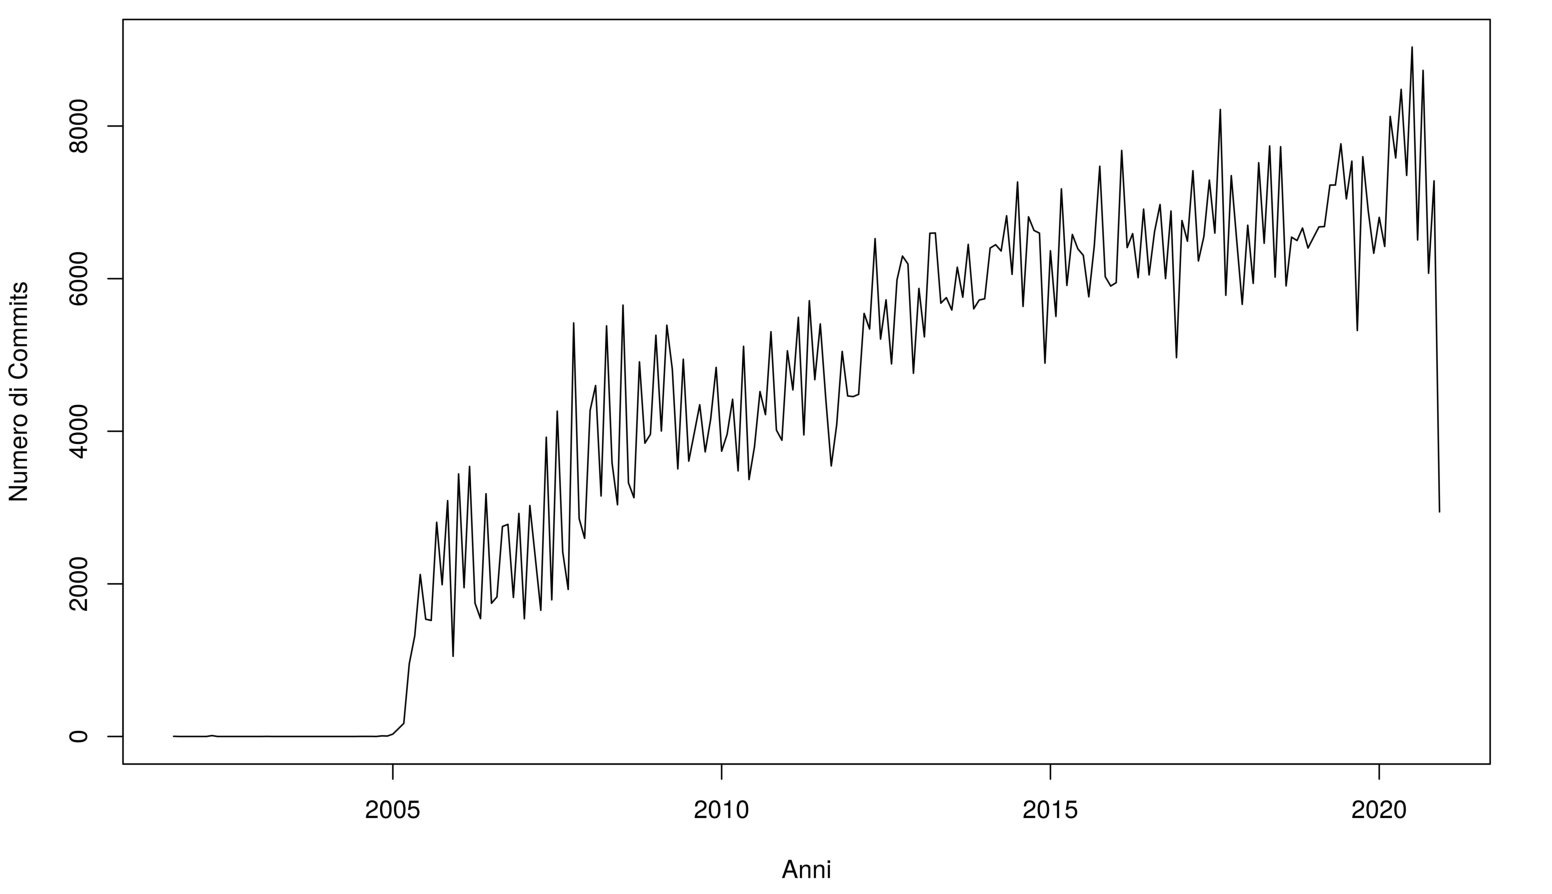
\includegraphics[scale=0.7]{imgs/ts_plot_1.pdf}
	\vspace{-0.8cm}
\end{figure}
\noindent
Inoltre, abbiamo un netto calo di commits nel mese di Dicembre 2020. Potrebbe
essere dovuto al fatto che ancora non abbiamo tutti i dati disponibili sino
all'ultimo giorno del mese: dobbiamo infatti tenere in considerazione che molti
sviluppatori tengono i propri commits in locale ed eseguono il \texttt{push}
sulla repository remota solamente a implementazione terminata. Dopo la pulizia:
\begin{figure}[H]
	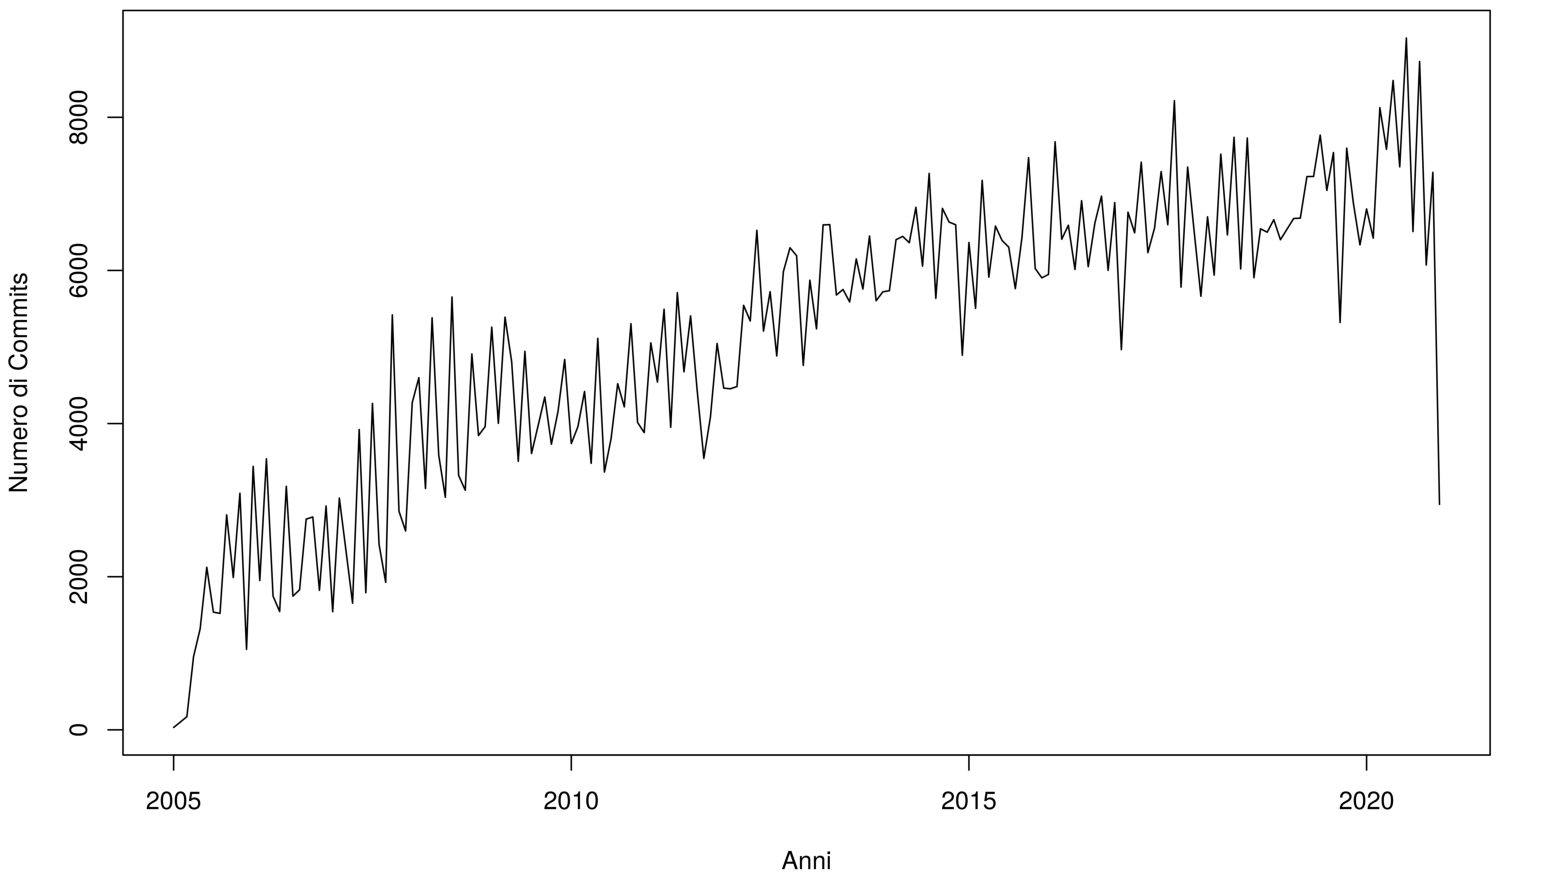
\includegraphics[scale=0.6]{imgs/ts_plot_2.pdf}
	\vspace{-1.0cm}
\end{figure}
\begin{lstlisting}[language=bash,basicstyle=\scriptsize,tabsize=2,frame = single]
> start(data_ts)	[1] 2005    1
> end(data_ts)		[1] 2020   12
> frequency(data_ts)	[1] 12
\end{lstlisting}
La funzione di autocorrelazione conferma la presenza di un Trend ascendente, non
sembra per\`o evidenziare alcuna stagionalit\`a.
\clearpage
\begin{figure}[H]
	\vspace{-1.5cm}
	\hspace{-0.5cm}
	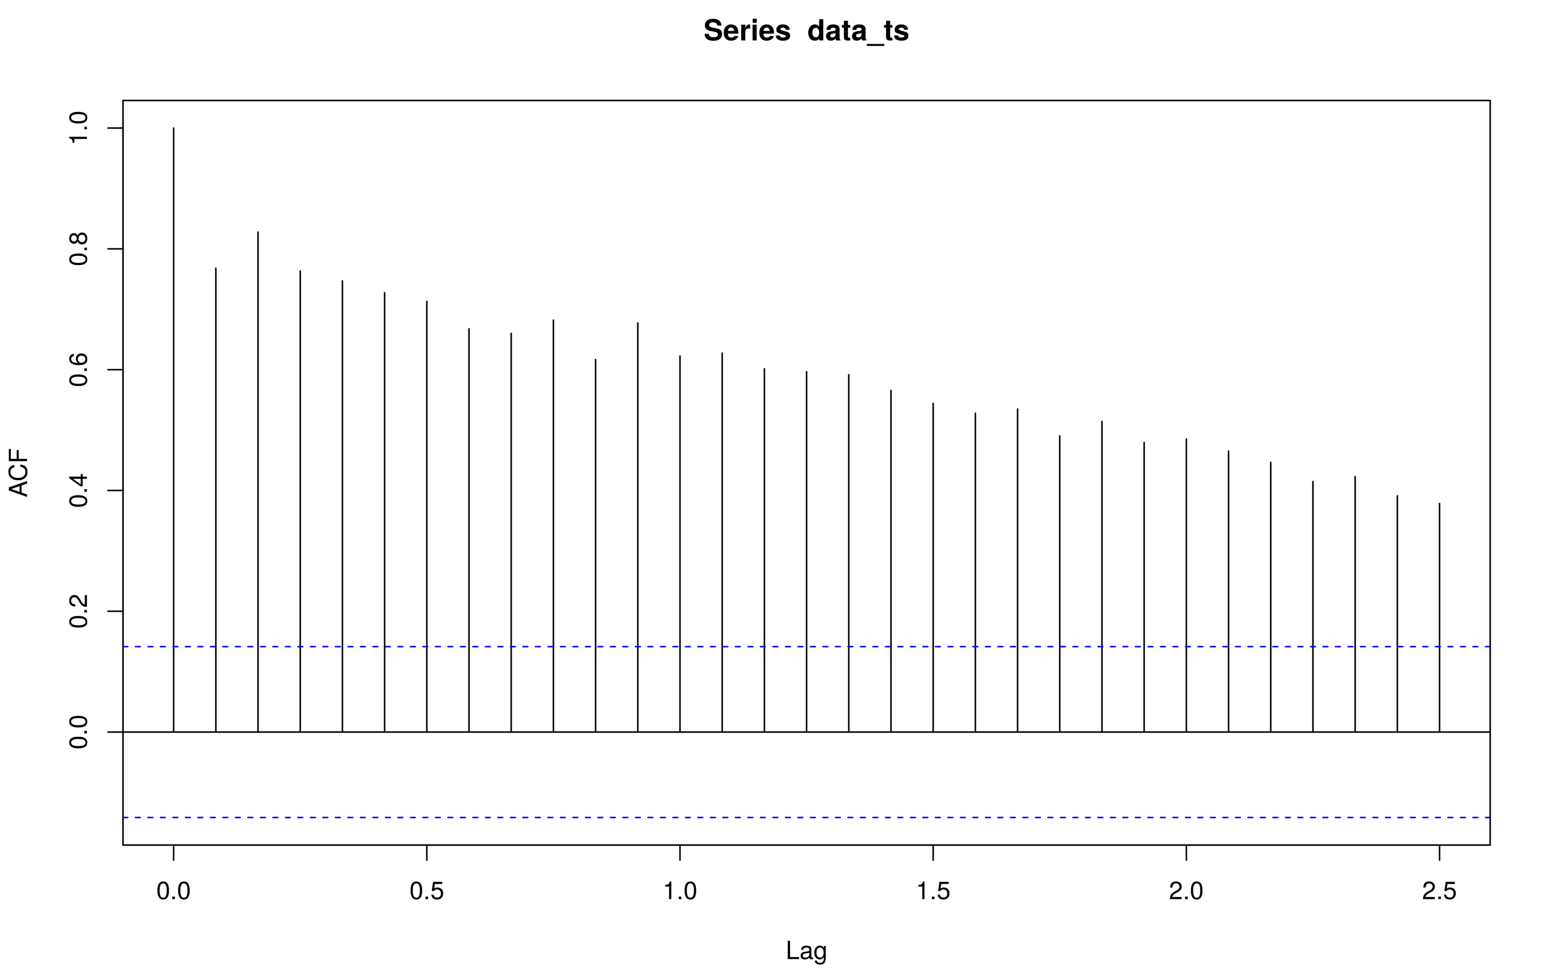
\includegraphics[scale=0.63]{imgs/acf.pdf}
\end{figure}
\noindent
Non era proprio quello che mi aspettavo dato che lo sviluppo di software, in
particolare il Kernel Linux, \`e una attivit\`a umana, di gruppo, e pertanto con
caratteri di stagionalit\`a. Inoltre, stiamo esaminando dati ragruppati per anno
su base mensile. \textbf{Ci sarebbero quindi i presupposti per riuscire a
catturare almeno una stagionalit\`a annuale}. Il mio sospetto \`e che il forte
Trend ascendente abbia nascosto la stagionalit\`a (dal 2005 al 2020 il numero di
commits mensili \`e aumentato da poche decine a picchi di circa $10000$). Provo
a investigare pi\`u a fondo.
\vspace{-0.4cm}
\begin{figure}[H]
	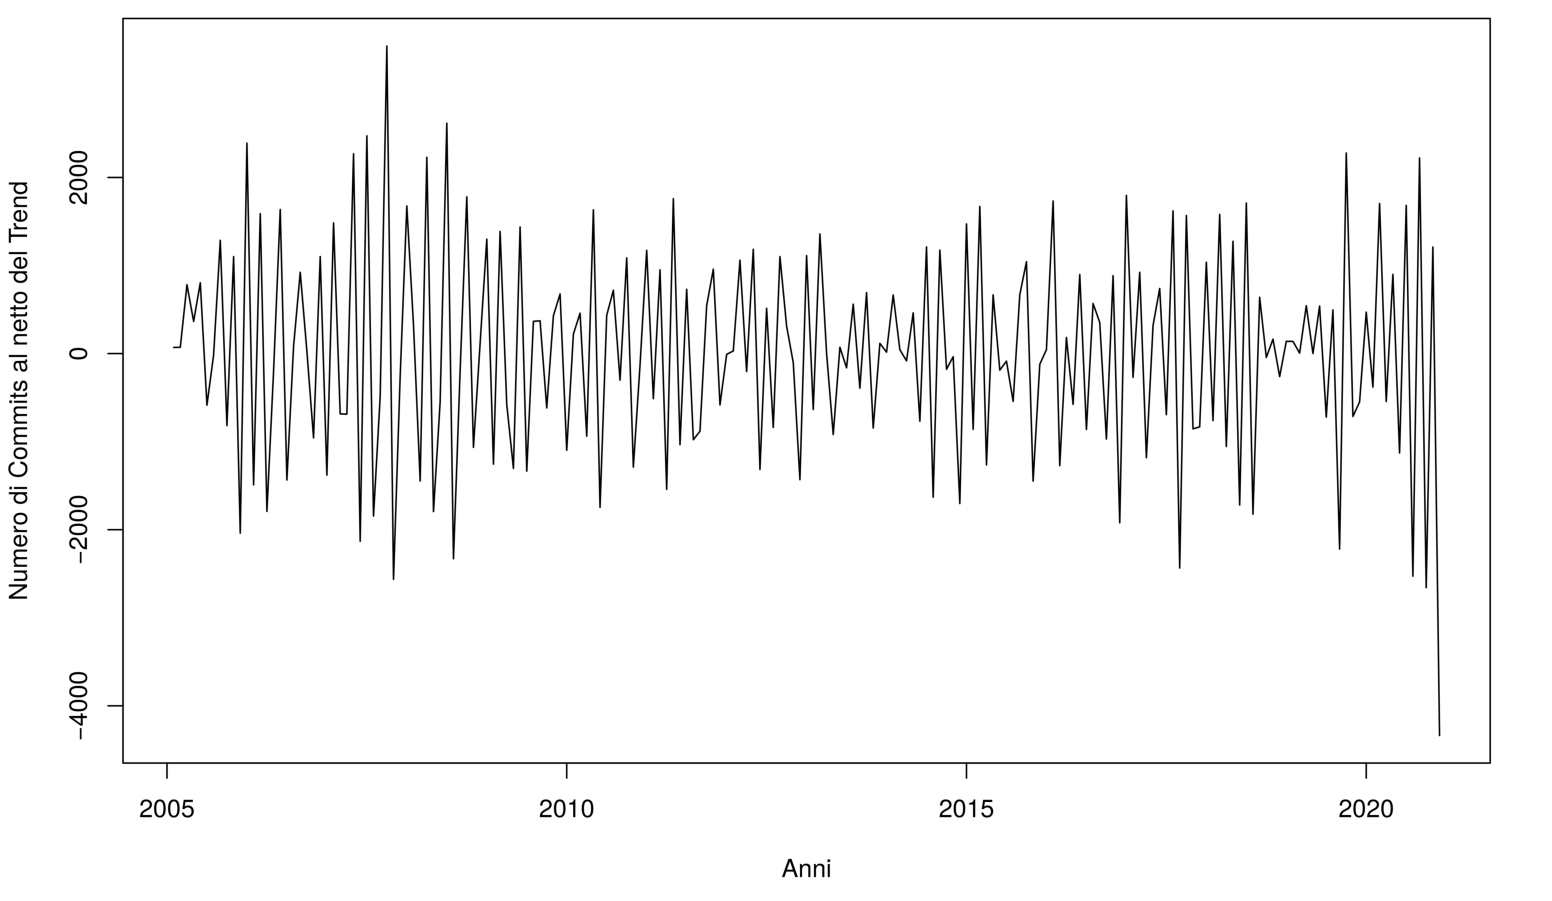
\includegraphics[scale=0.6]{imgs/diff.pdf}
	\vspace{-0.9cm}
\end{figure}
\noindent
Anche osservando i nostri dati al netto della progressione aritmetica
del Trend, vediamo oscillazioni senza alcuna struttura. Nuovamente, non sembra
ci sia alcuna componente di stagionalit\`a.
\clearpage
\begin{figure}[H]
	\vspace{-1.5cm}
	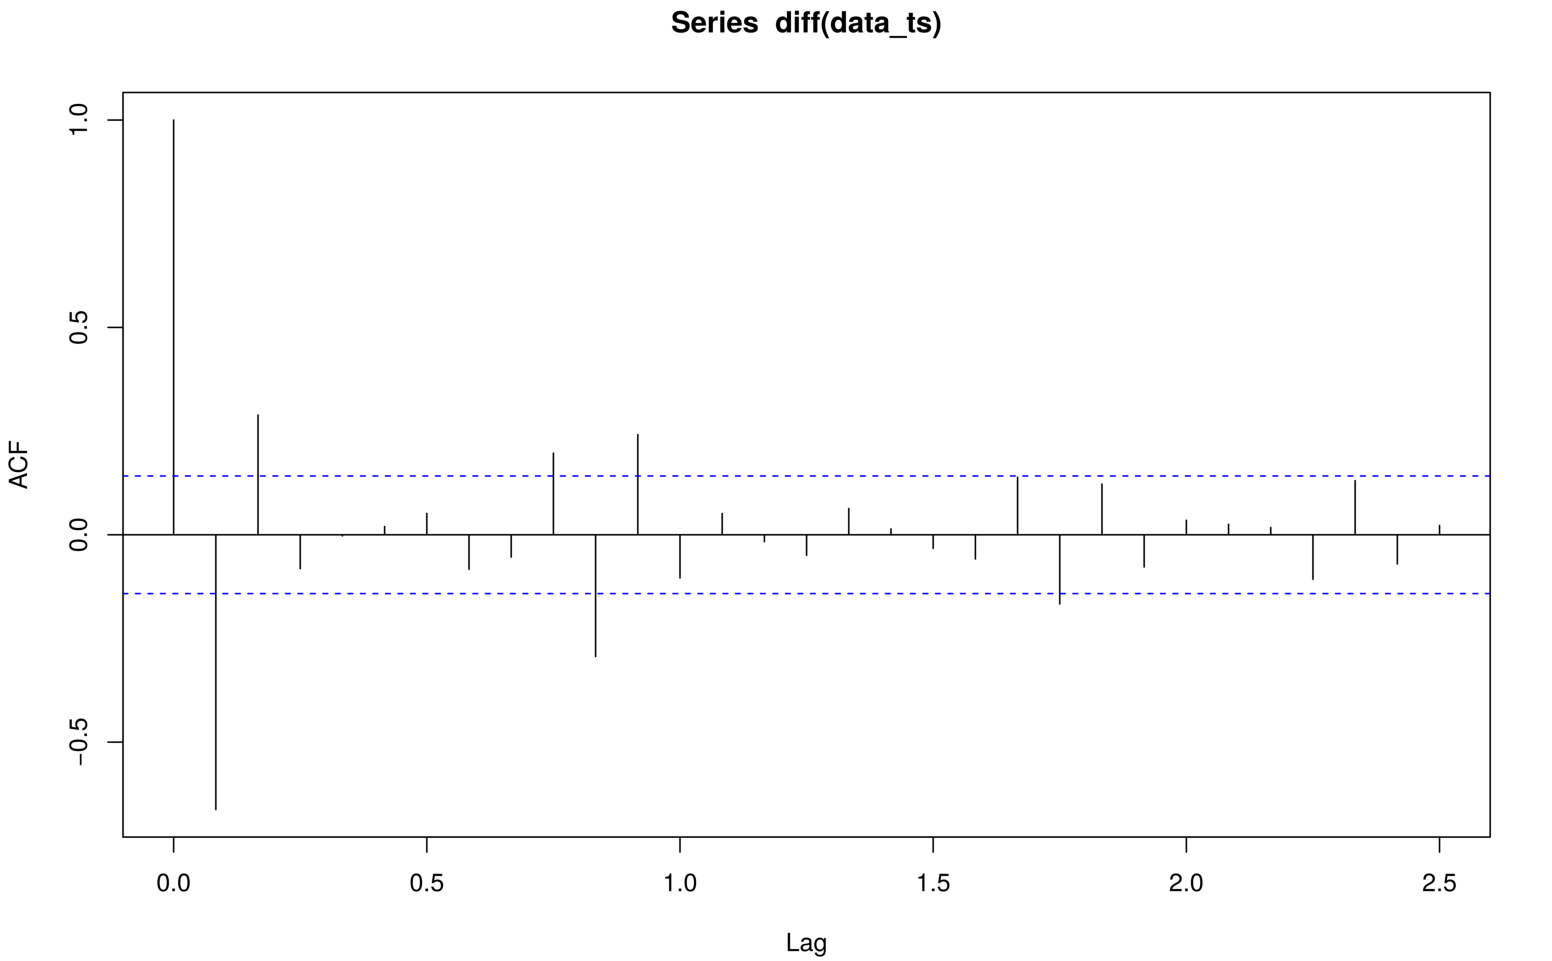
\includegraphics[scale=0.6]{imgs/acf_diff.pdf}
	\vspace{-0.8cm}
\end{figure}
\noindent
Notiamo anche che la variabilit\`a del numero di commit per mese, durante i
16 anni presi in considerazione, \`e elevata.
\begin{figure}[H]
	\vspace{-0.3cm}
	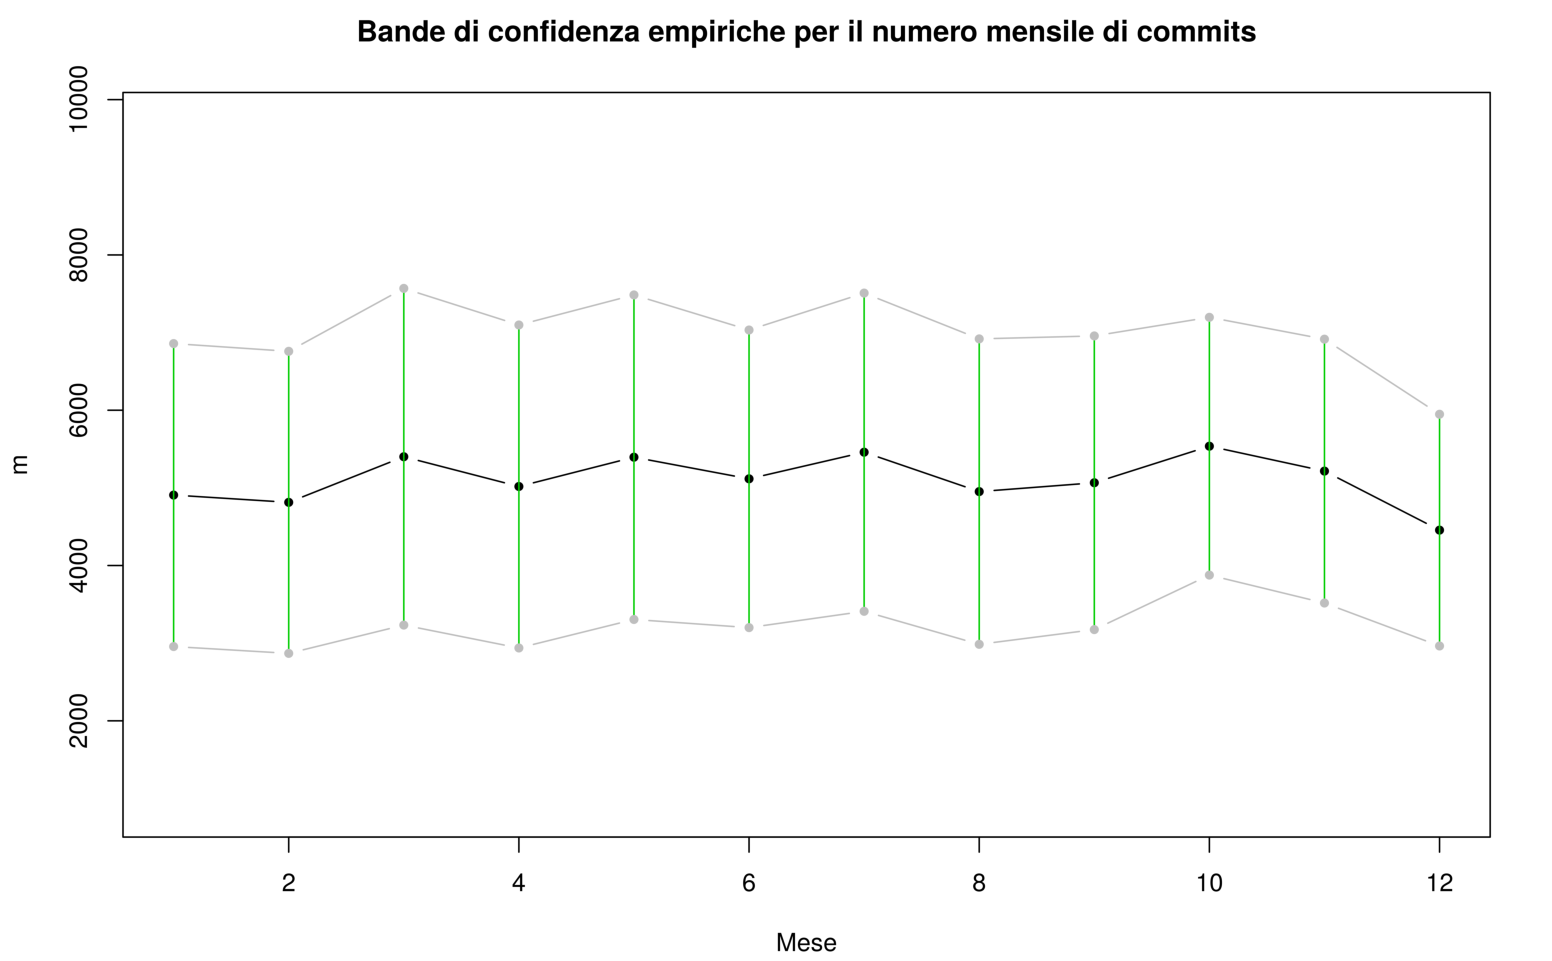
\includegraphics[scale=0.6]{imgs/variance.pdf}
	\vspace{-0.9cm}
\end{figure}

\section{Decomposizione}
L'analisi, sino ad ora, non ci suggerisce la presenza di stagionalit\`a, almeno
con periodo 12 (annuale). Tuttavia, avendo un periodo suggerito dal fenomeno,
possiamo comunque tentare una decomposizione per toglierci ogni dubbio.
C'\`e un Trend abbastanza chiaro che ben cattura l'andamento della nostra serie.
Notiamo che il rumore non \`e strutturato. Approfondiremo l'analisi dei residui
in seguito. \textbf{Bisogna sottolineare che il rumore \`e chiaramente pi\`u
ampio della componente stagionale.}
\clearpage
\begin{figure}[H]
	\vspace{-1.5cm}
	\hspace{-1.5cm}
	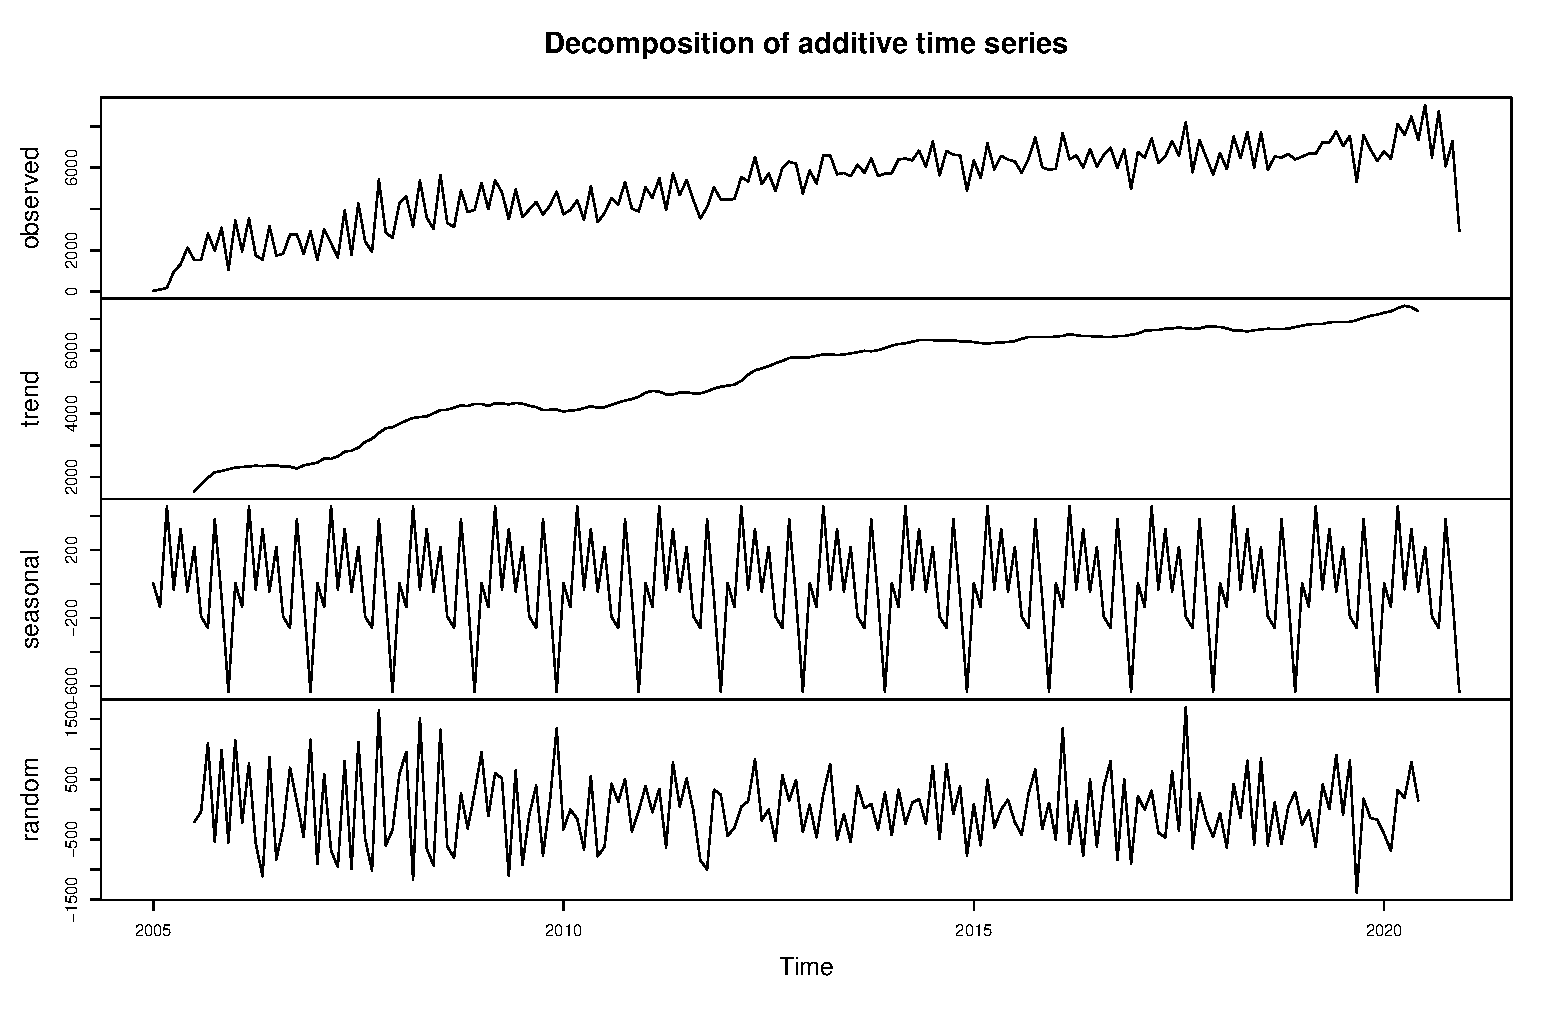
\includegraphics[scale=0.7]{imgs/decompose_additive.pdf}
	\vspace{-0.9cm}
\end{figure}
\begin{figure}[H]
	\vspace{-0.9cm}
	\hspace{-1.5cm}
	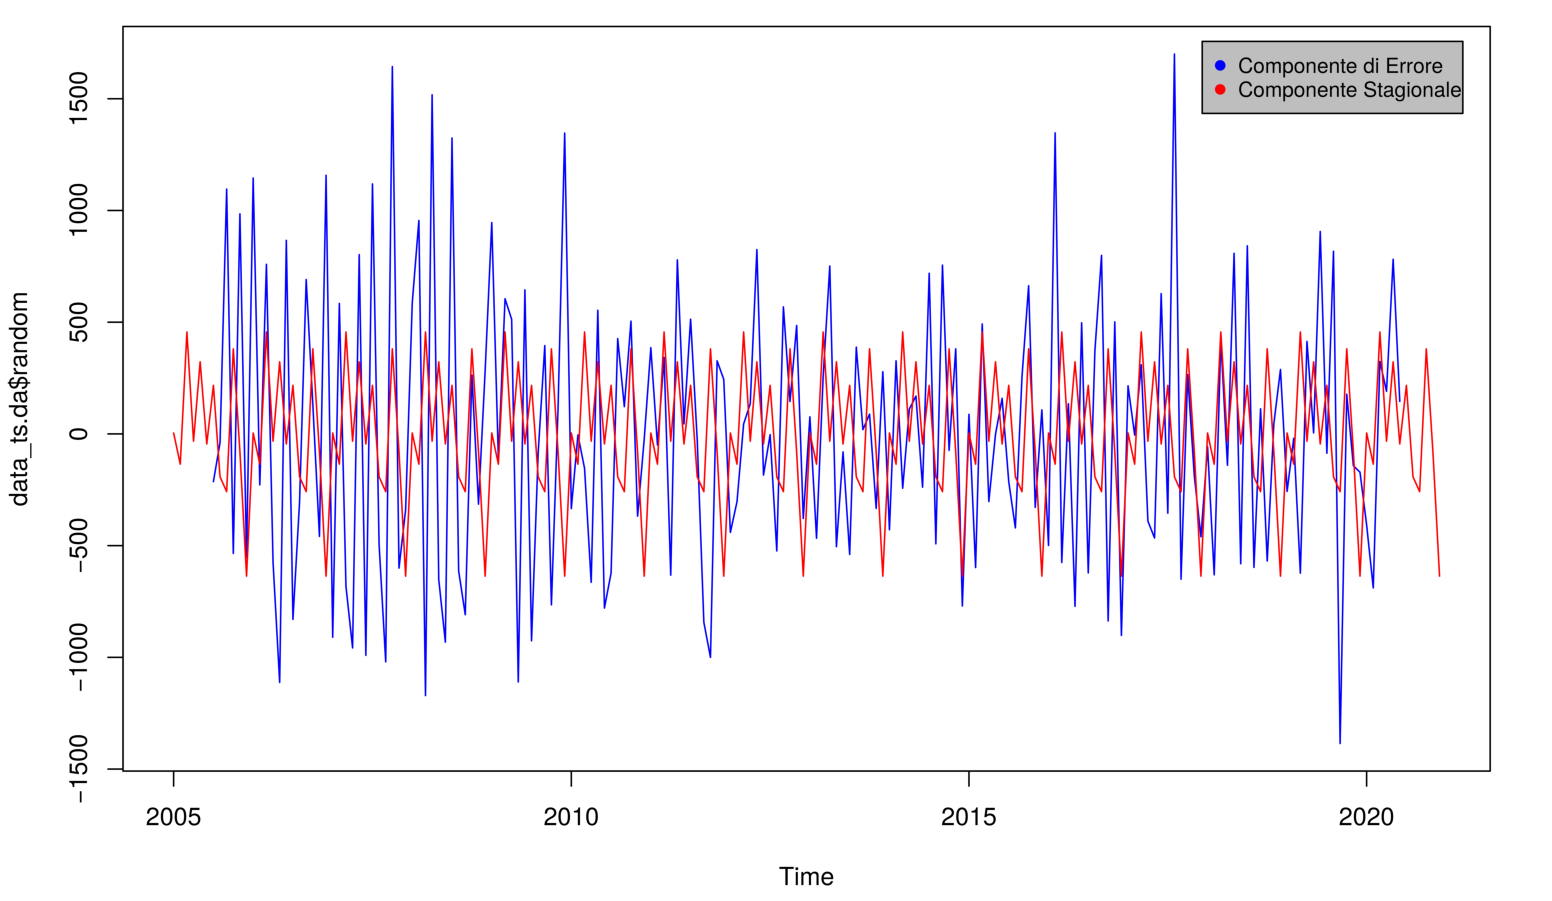
\includegraphics[scale=0.7]{imgs/random_seasonal.pdf}
	\vspace{-0.9cm}
\end{figure}
\noindent
Abbiamo sbagliato tipo di decomposizione? Direi di no: se osserviamo infatti il
grafico della decomposizione, notiamo  inizialmente un Trend pi\`u piccolo, poi
cresce, ma a questo non corrisponde una analoga variabilit\`a dei residui.
\textbf{La mia conclusione \`e che la componente di stagionalit\`a o \`e
decisamente trascurabile oppure \`e non uniforme.}

\subsection{Analisi dei residui}
L'analisi dei residui ci fornisce una ulteriore conferma di quanto osservato
sino ad ora: la decomposizione additiva \`e quella pi\`u appropiata, certamente
i residui additivi mostrano minore struttura, \textbf{quindi la componente
stagionale non era stata nascosta da una decomposizione errata, pertanto o non
\`e presente o comunque decisamente trascurabile, oppure non ha un andamento
uniforme}.
\begin{figure}[H]
	\vspace{-0.3cm}
	\hspace{-2.7cm}
	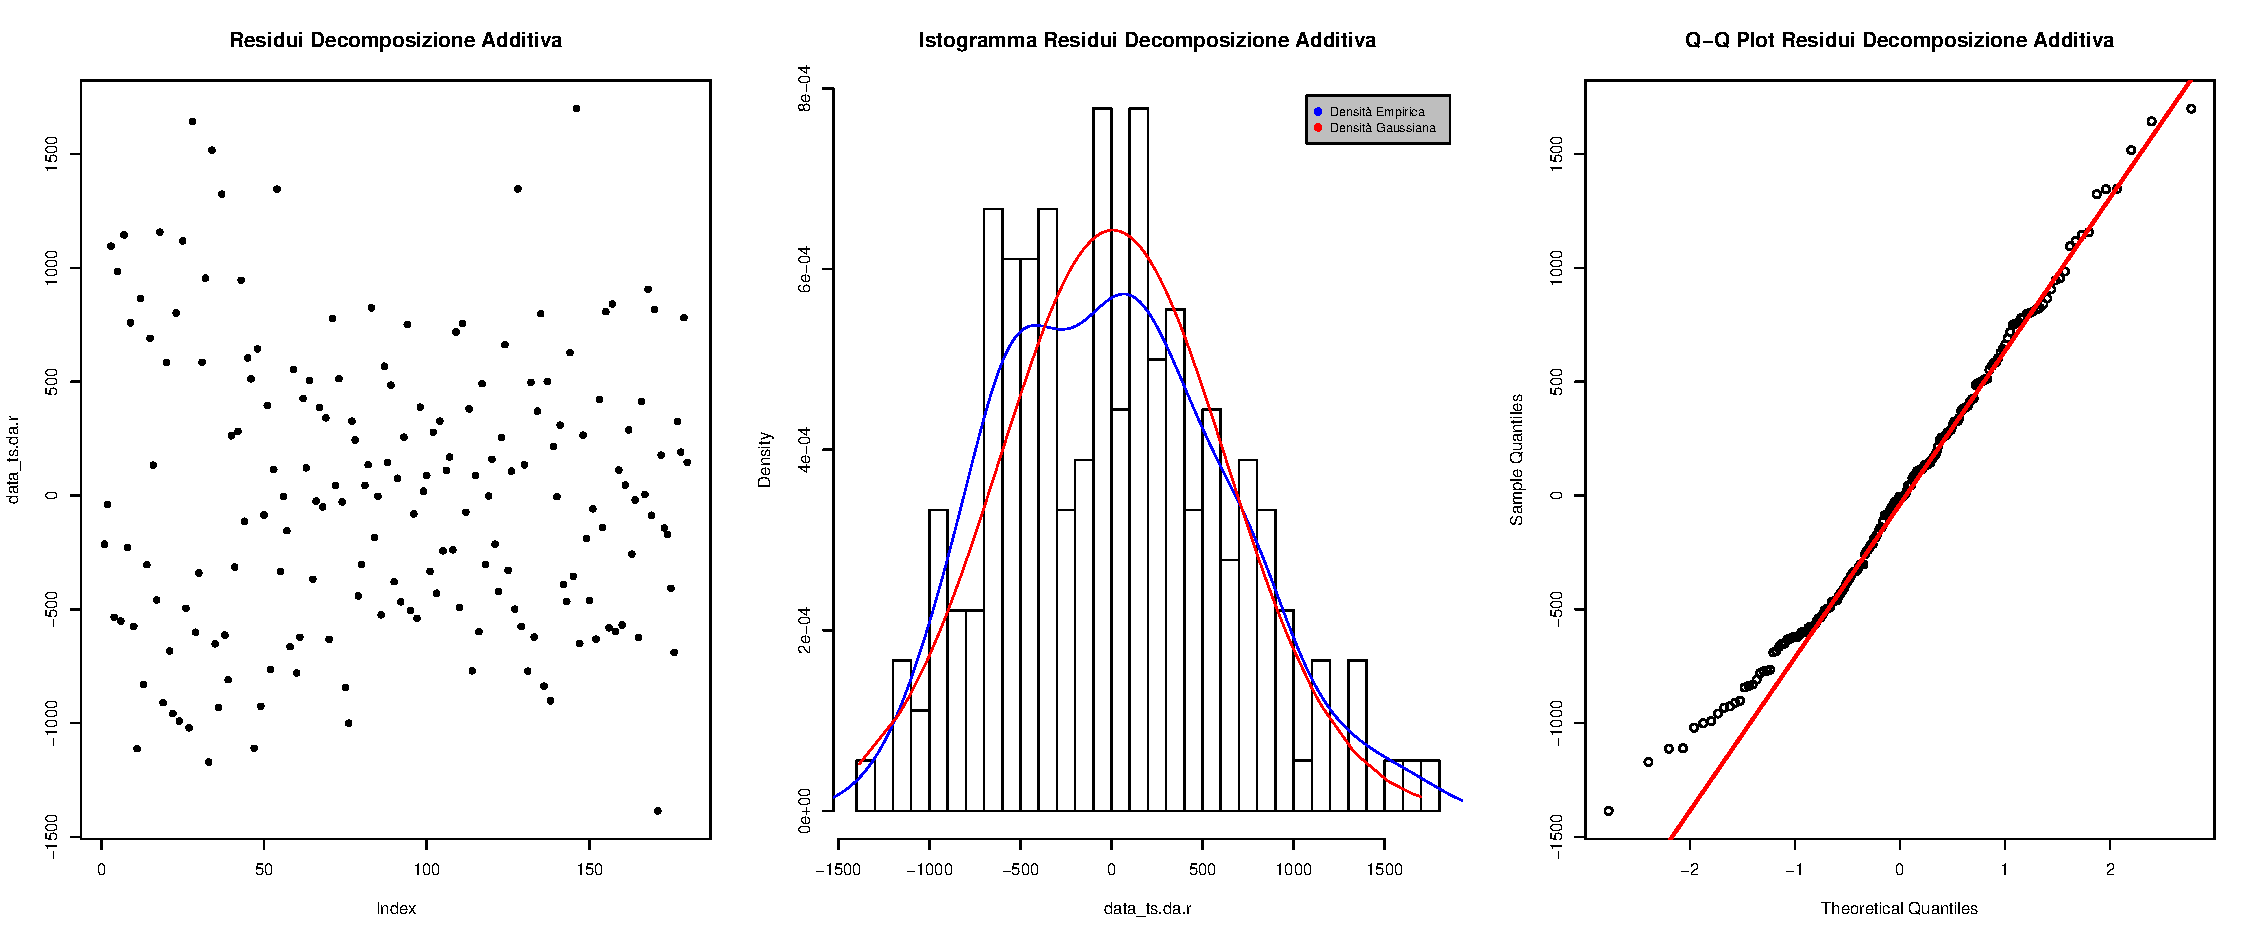
\includegraphics[scale=0.55]{imgs/additive_residuals.pdf}
\end{figure}
\begin{figure}[H]
	\vspace{-0.5cm}
	\hspace{-2.7cm}
	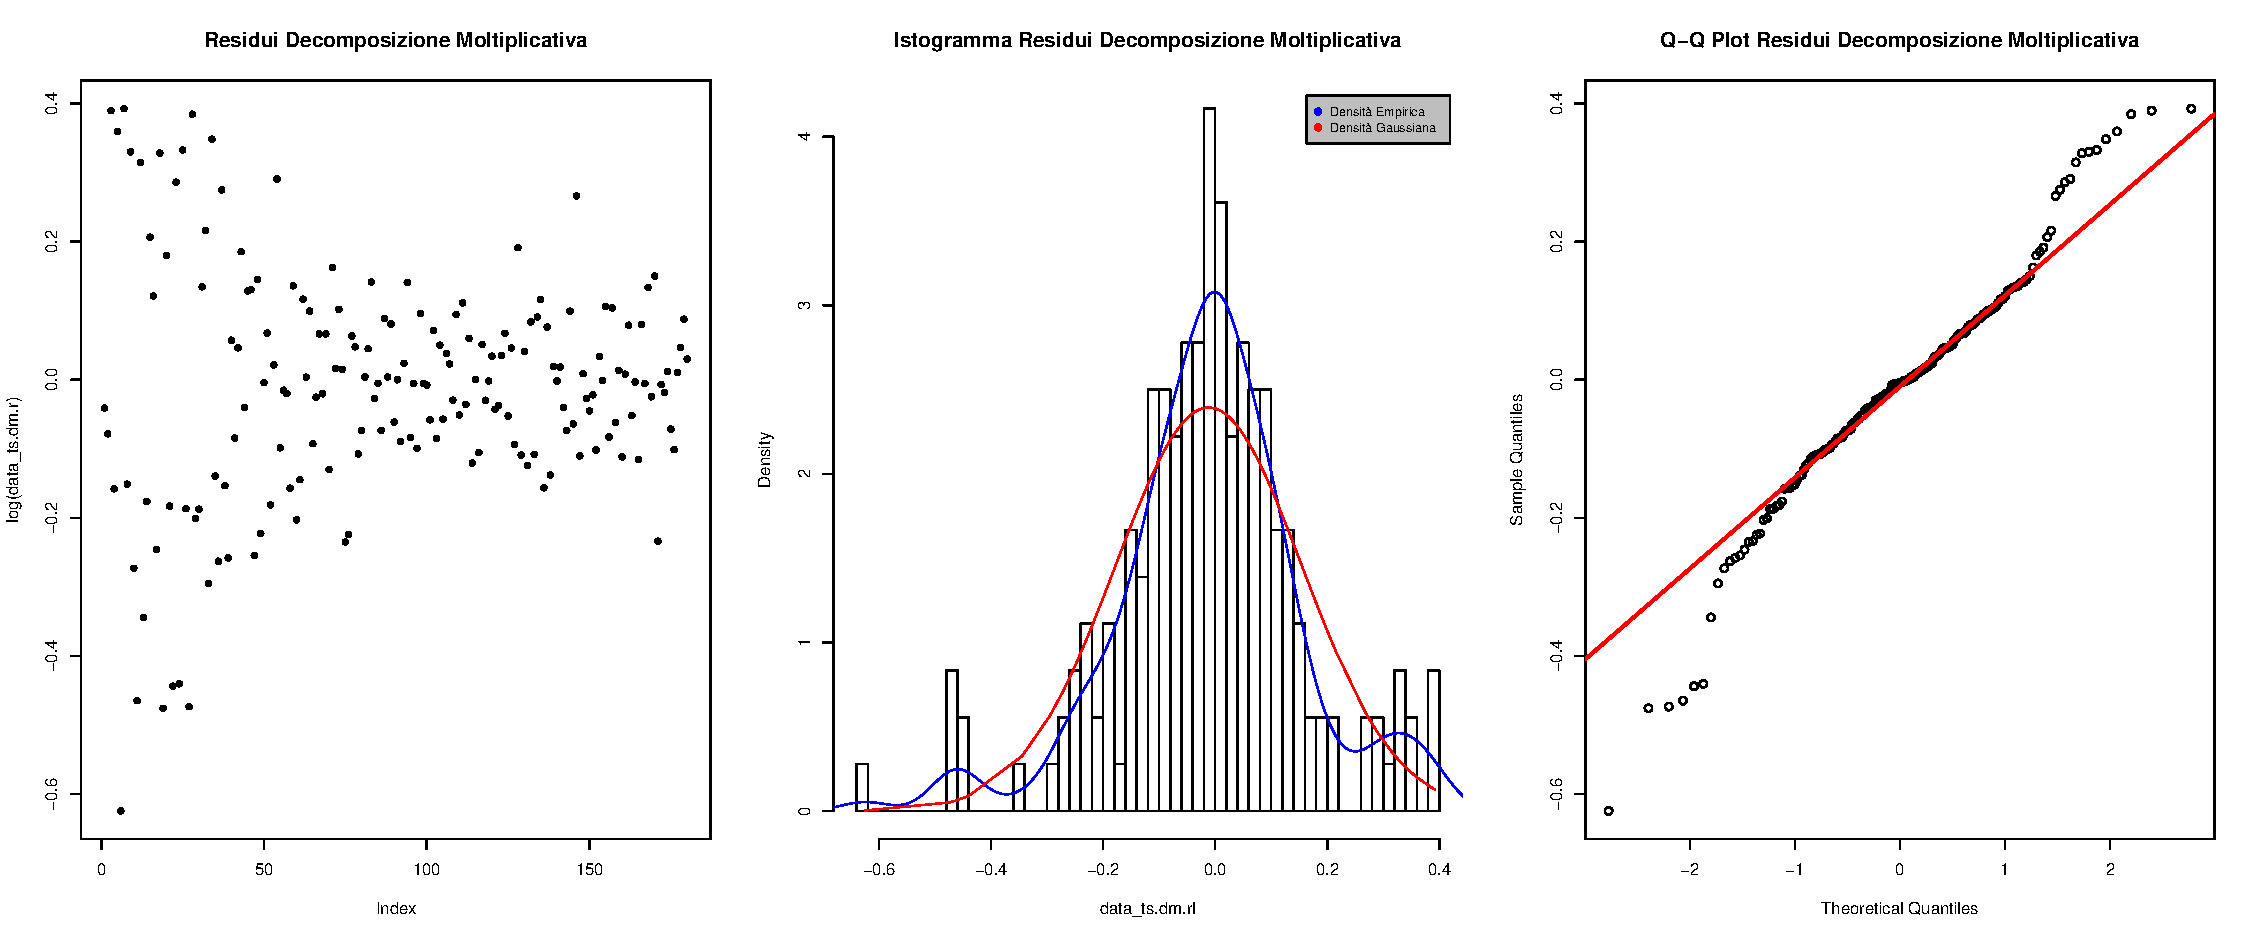
\includegraphics[scale=0.55]{imgs/multiplicative_residuals.pdf}
\end{figure}

\subsection{Decomposizione con stagionalit\`a non uniforme}
Guardando il grafico dell'andamento centrato a media nulla dei commits, mi viene
da pensare che ci sia una componente stagionale che per\`o varia da anno ad
anno. Ho quindi pensato di tentare una decomposizione con stagionalit\`a non
uniforme per vedere se si riesca ad estrarre quella componente di periodicit\`a
che il fenomeno ci suggerisce.
\clearpage
\begin{figure}[H]
\begin{center}
	\vspace{-1.5cm}
	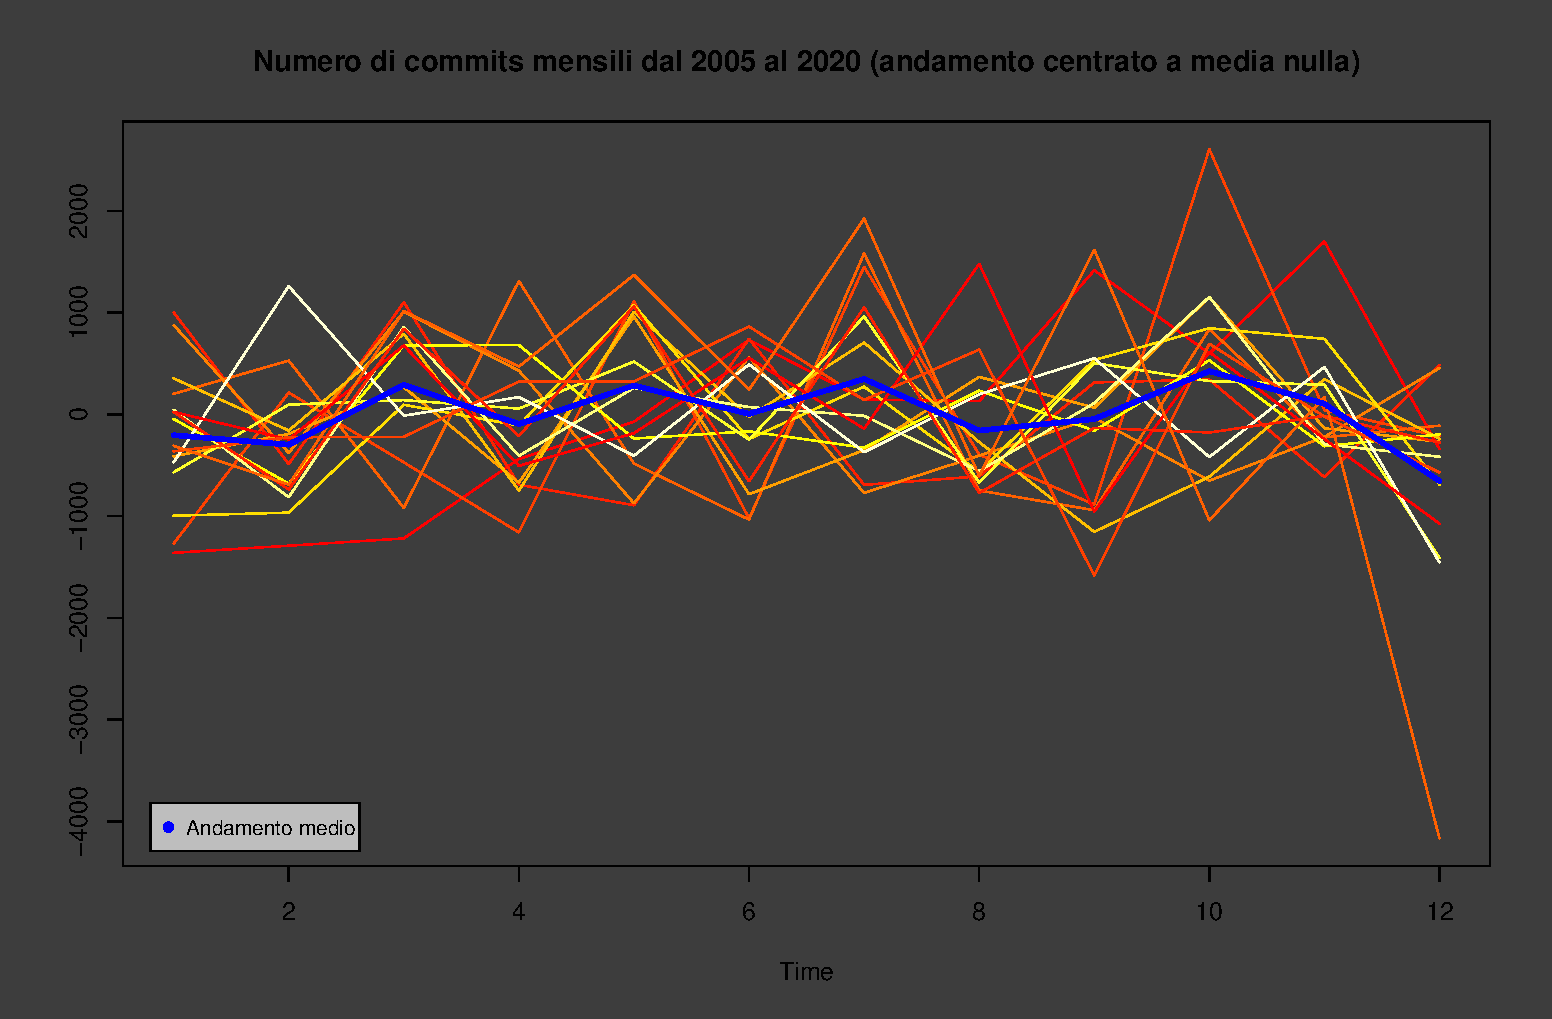
\includegraphics[scale=0.5]{imgs/heat_colors.pdf}
	\vspace{-0.5cm}
\end{center}
\end{figure}
\noindent
Con una scelta della dimensione della \texttt{seasonal window} pari a 3 si
ottiene una componente stagionale che ha una variabilit\`a significativa a
confronto con il Trend, e soprattutto maggiore di quella del rumore.
Questo ci mostra quindi che il fenomeno che ci troviamo ad analizzare ha
effettivamente \textbf{una componente di stagionalit\`a che per\`o evolve in
maniera molto rapida.} I metodi di analisi precedentemente utilizzati prendevano
in considerazione una finestra troppo ampia e l'analisi veniva quindi falsata
dai pattern di stagionalit\`a passati che non erano pi\`u rilevanti.
\begin{figure}[H]
	\vspace{-0.4cm}
	\hspace{-1.5cm}
	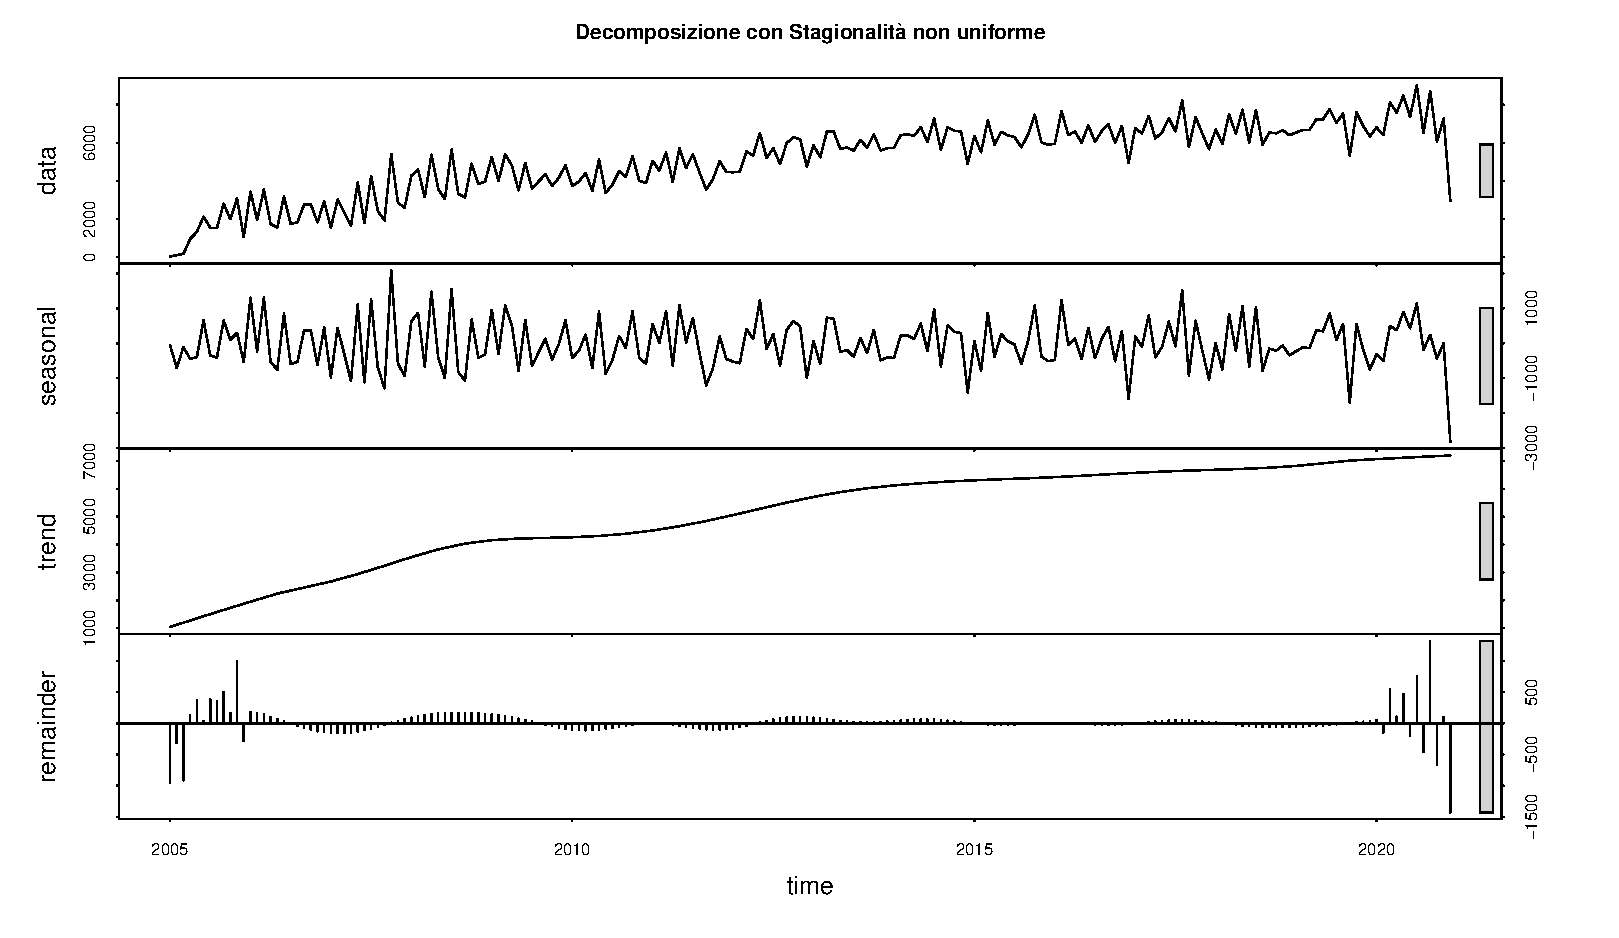
\includegraphics[scale=0.7]{imgs/stl.pdf}
\end{figure}
\section{Previsione}
Al termine di questa prima fase dianalisi, una delle considerazioni pi\`u
importanti che dobbiamo tenere a mente \`e che sicuramente lo sviluppo del
codice sorgente del Kernel Linux \`e una attivit\`a umana e di gruppo; tuttavia,
si distingue dalle altre in quanto gli individui che vi partecipano sono
volontari; di conseguenza il numero di sviluppatori, e quindi anche quello dei
commits, \`e affetto da una variabilit\`a significativa ed \`e anche difficile
da prevedere. Non solo, questi commits provengono anche da grosse multinazionali
(Oracle, RedHat, Google, IBM, Facebook, Amazon), e da altri enti come NASA,
CERN, Dipartimento della Difesa degli Stati Uniti, ecc\dots. Il numero di
commits pu\`o quindi variare anche a seconda delle necessit\`a di sviluppo
software interne a questi enti. \textbf{In fase di previsione quindi dobbiamo
tenere a mente che queste variazioni non sono propriamente dovute ad un fenomeno
strutturale, ma piuttosto ad un fenomeno che contiene ampie componenti di
aleatoriet\`a}.

\subsection{Holt-Winters}
Ho valutato per mezzo di autovalutazione un modello a smorzamento esponenziale,
uno a smorzamento esponenziale con Trend e uno a smorzamento esponenziale con
Trend e Stagionalit\`a.
\begin{figure}[H]
	\vspace{-0.4cm}
	\hspace{-1.5cm}
	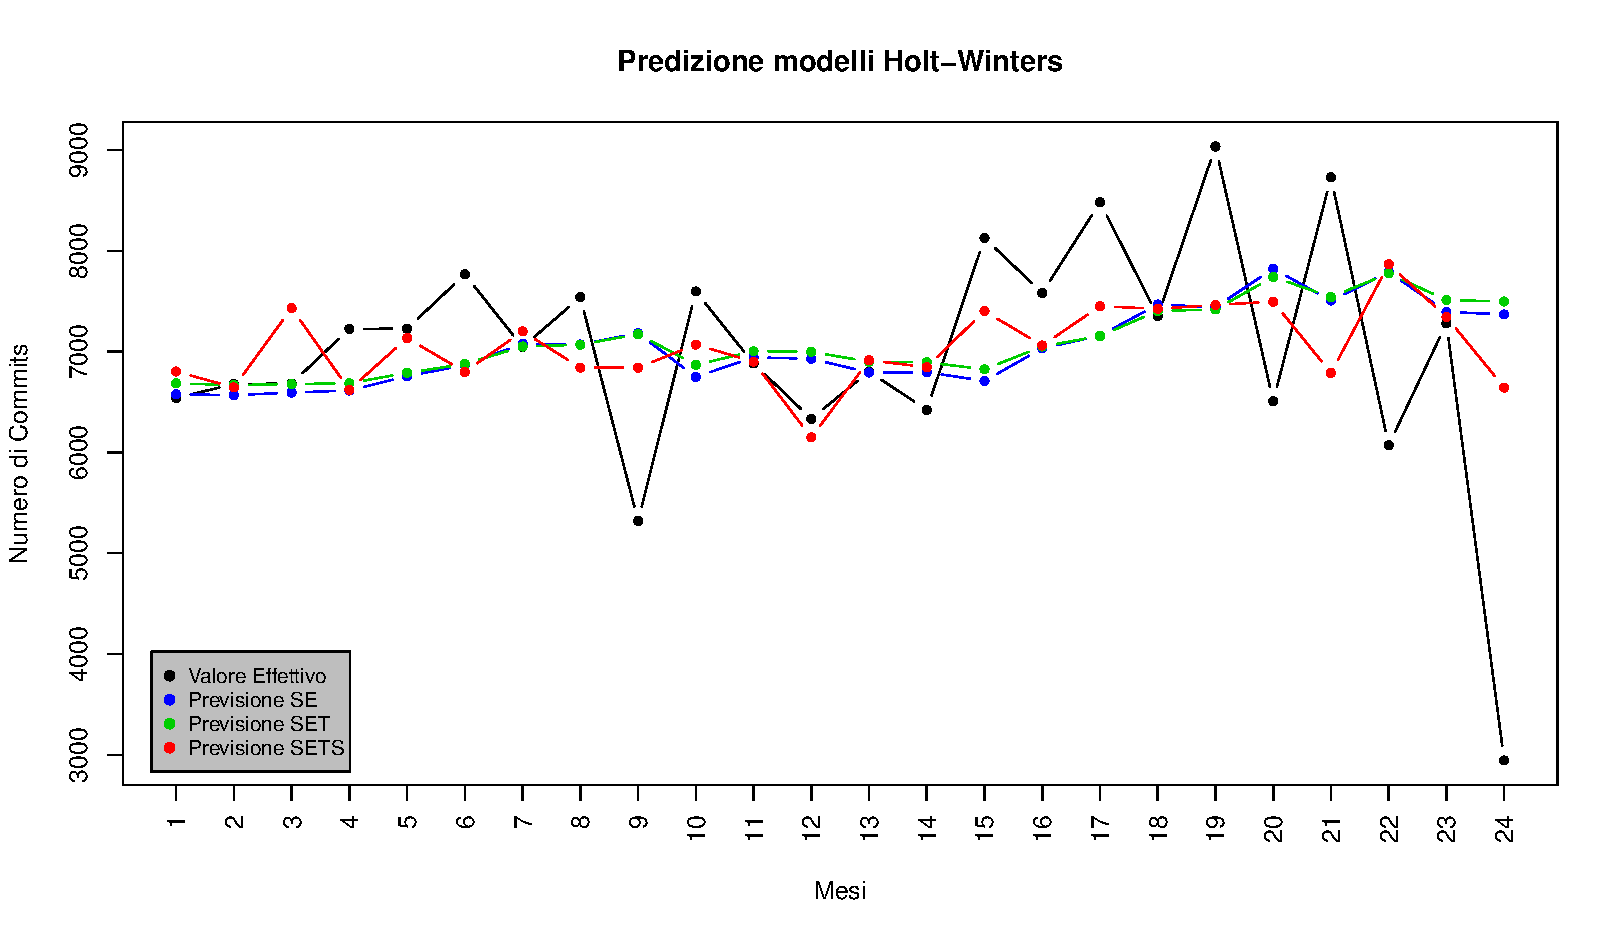
\includegraphics[scale=0.66]{imgs/HW_predict.pdf}
\end{figure}
\vspace{-0.6cm}
\noindent
In quanto a previsioni, non possiamo certamente dire che ci sia un modello che
faccia nettamente meglio degli altri. Per quanto riguarda i valori di errore
invece, il modello a smorzamento esponenziale con Trend e Stagionalit\`a
sembrerebbe fare leggermente meglio. Dobbiamo tenere in considerazione per\`o
che gli errori aumentano per quanto riguarda gli ultimi mesi del 2020. In
effetti, \`e possibile che molti commits relativi a questi mesi non siano ancora
stati accettati nella mainline del Kernel Linux (la repository
\textbf{torvalds/linux} dalla quale abbiamo estratto i dati di partenza). Questo
perch\`e, per assicurarsi che niente possa rompere il Kernel Linux, il processo
di approvazione di un commit \`e lungo: ogni modifica deve essere approvata da
pi\`u di uno degli sviluppatori facenti parte della TOP 10.
\begin{figure}[H]
	\vspace{-1.5cm}
	\hspace{-1.5cm}
	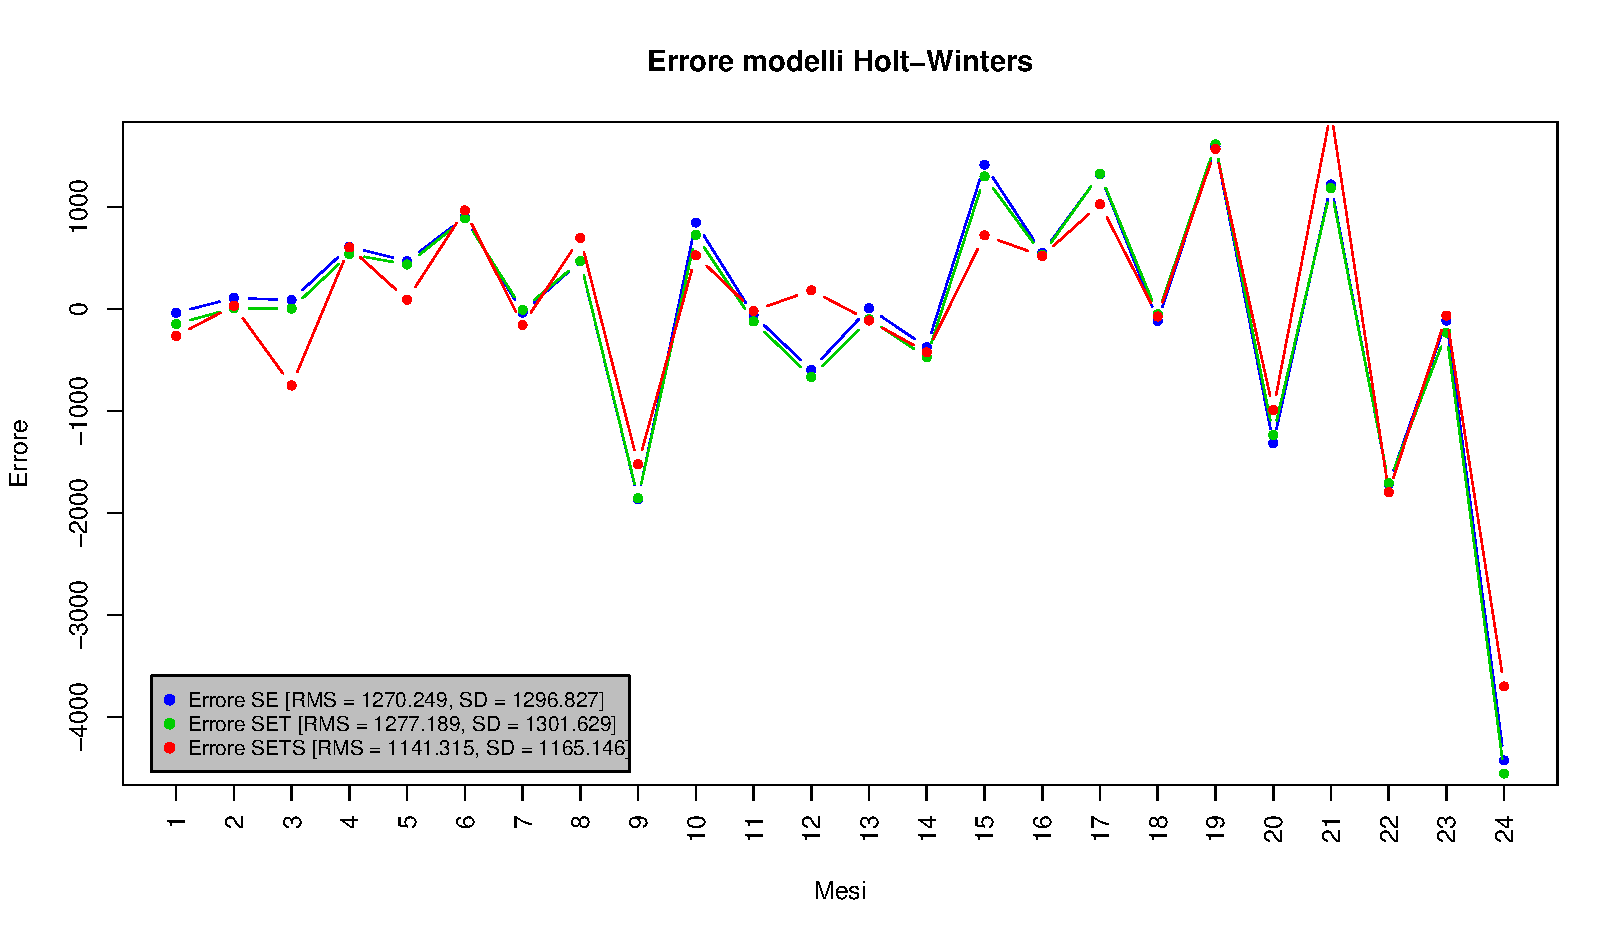
\includegraphics[scale=0.66]{imgs/HW_residuals.pdf}
	\vspace{-1.2cm}
\end{figure}
\noindent
Ci sono stati degli errori di ottimizzazione dei parametri per quanto riguarda
il modello Holt-Winters che per\`o abbiamo ignorato.\\
Data la nostra conoscenza del fenomeno, e i risultati ottenuti in fase di
analisi delle componenti di Trend e Stagionalit\`a, il modello che preferisco
\`e quello a smorzamento esponenziale con Trend:
\begin{figure}[H]
	\vspace{-0.4cm}
	\hspace{-1.5cm}
	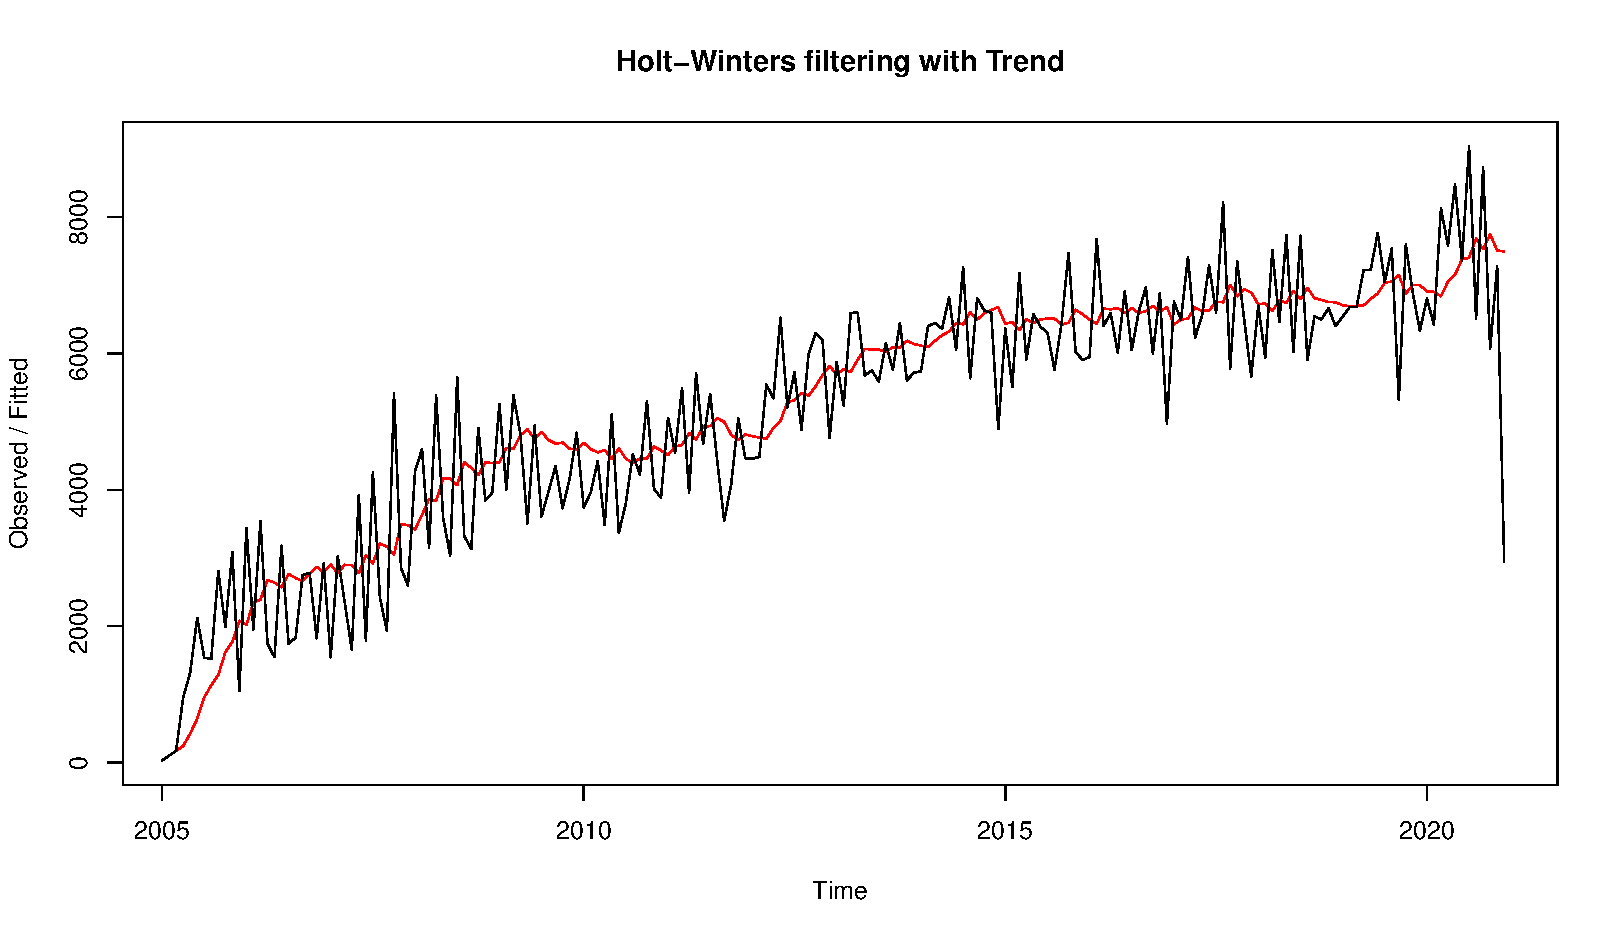
\includegraphics[scale=0.65]{imgs/HW_trend.pdf}
	\vspace{-1.0cm}
\end{figure}
\noindent
Siamo soddisfatti anche della normalit\`a dei residui di tale modello:
\begin{lstlisting}[language=bash,basicstyle=\scriptsize,tabsize=2,frame = single]
> shapiro.test(data_ts.set.r)

	Shapiro-Wilk normality test

data:  data_ts.set.r
W = 0.98895, p-value = 0.1504
\end{lstlisting}
\begin{figure}[H]
	\vspace{-1.5cm}
	\hspace{-2.7cm}
	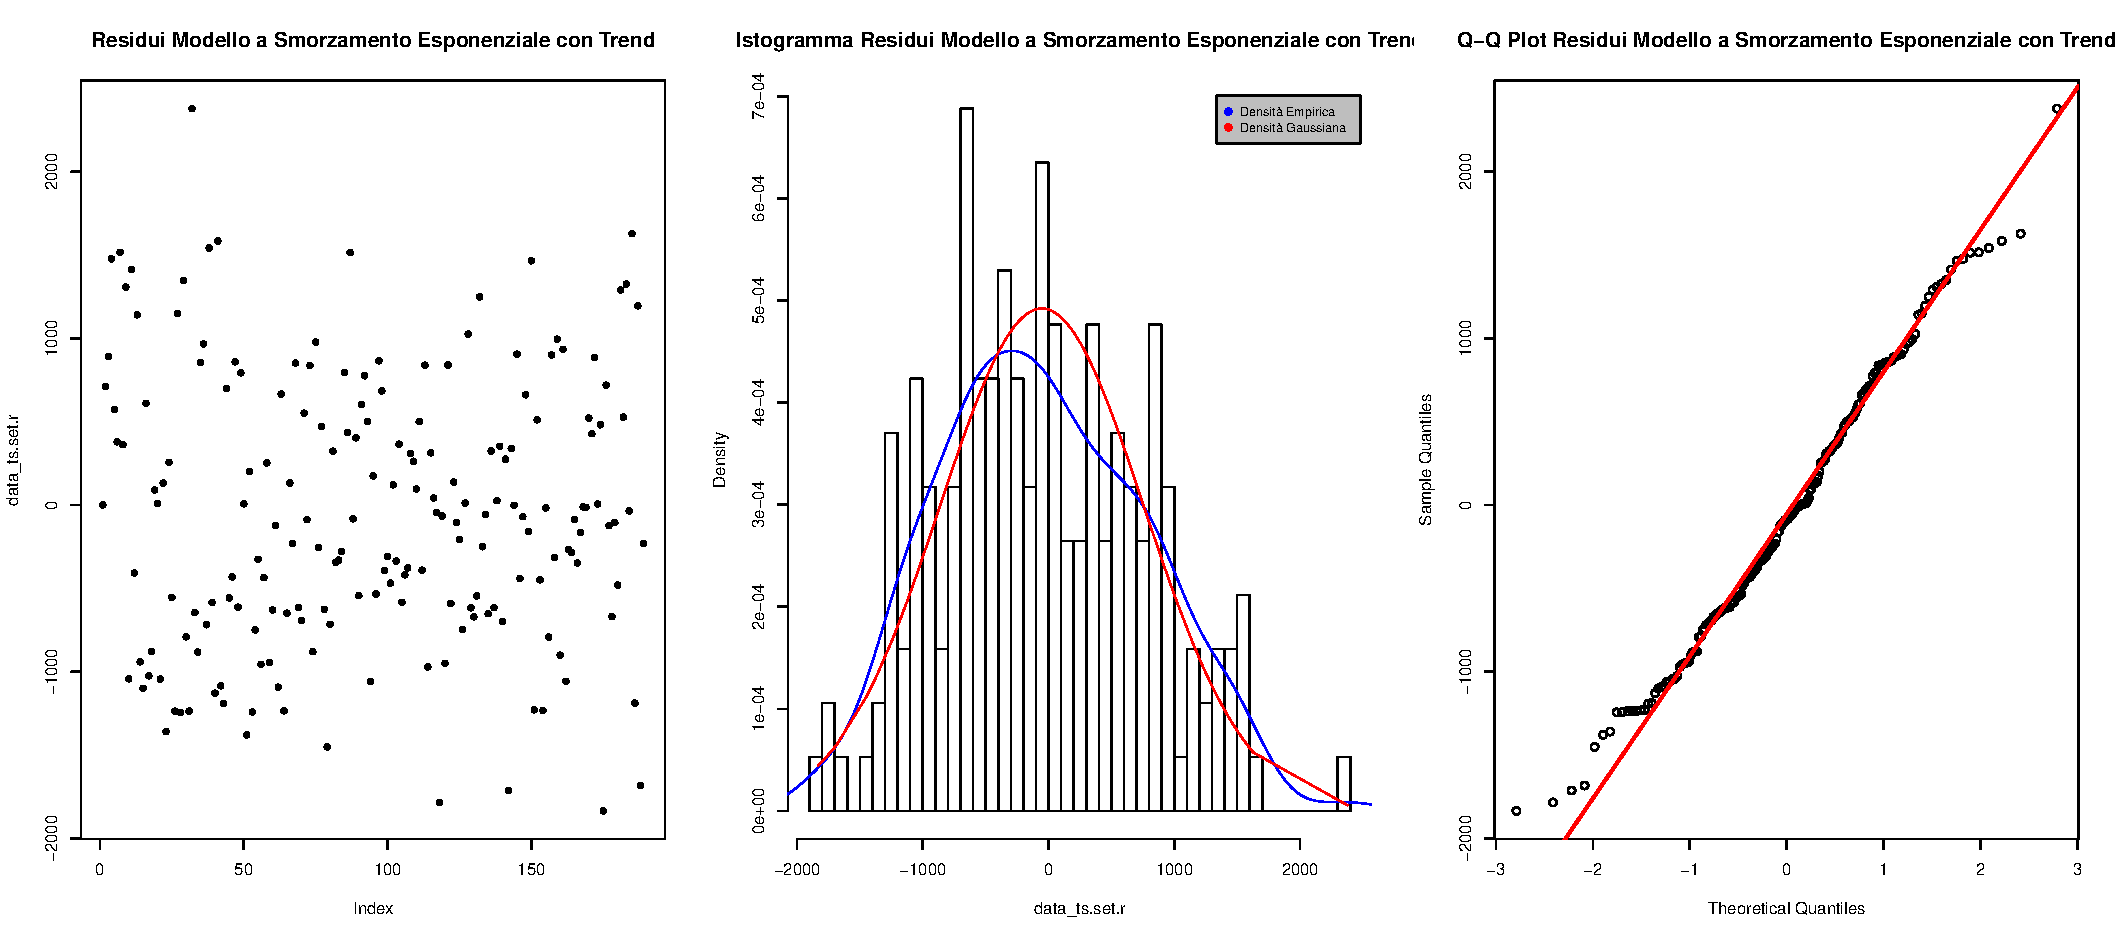
\includegraphics[scale=0.57]{imgs/HW_residuals_normality.pdf}
\end{figure}

\subsection{Autoregressione con il metodo dei minimi quadrati}
La nostra conoscienza del fenomeno, i risultati raggiunti in termini della
stagionalit\`a, la funzione di autocorrelazione e di autocorrelazione parziale
ci suggeriscono che ci siano effettivamente i presupposti per procedere con
l'analisi di un modello autoregressivo.
\begin{figure}[H]
	\vspace{-0.3cm}
	\hspace{-1.5cm}
	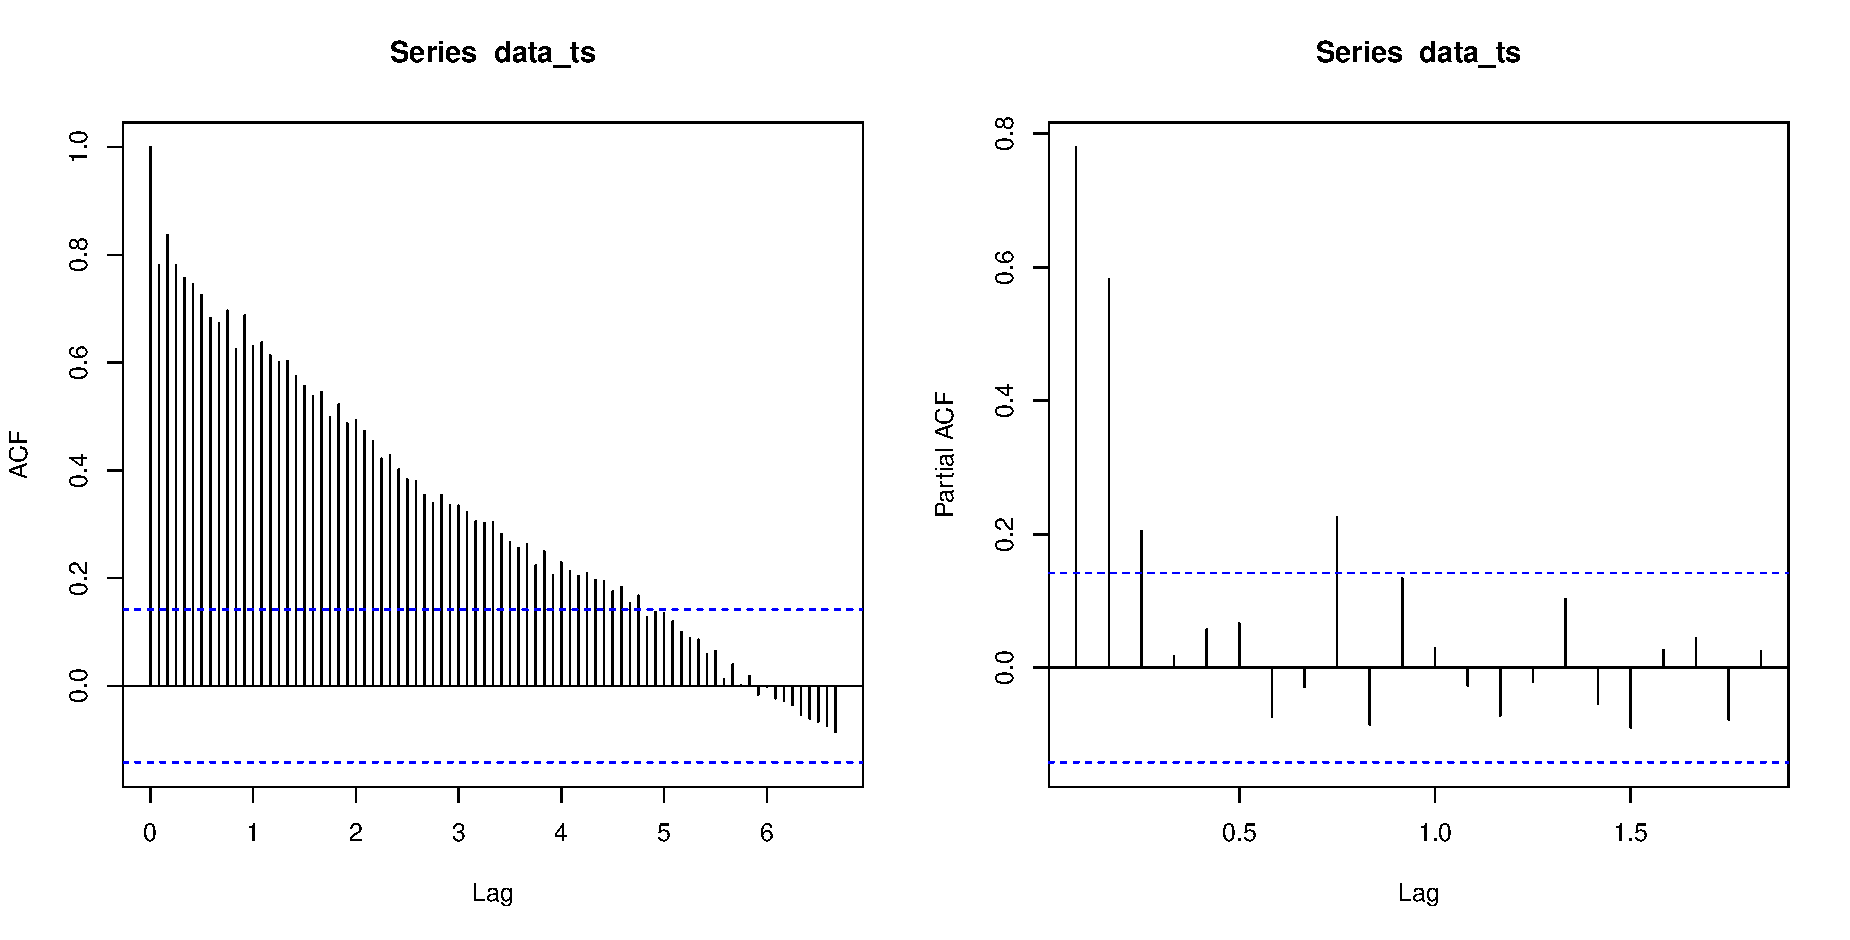
\includegraphics[scale=0.57]{imgs/acf_pacf.pdf}
	\vspace{-1.0cm}
\end{figure}
\noindent
Questo modello, a differenza di quello di Holt-Winters che si basava
principalmente sul Trend, dovrebbe riuscire a catturare questo fenomeno
tempo-variante che porta ad una elevata variabilit\`a del numero di commits. Ho
scelto quindi di valutare un modello di Autoregressione con il metodo dei minimi
quadrati per riuscire a catturare la parte non stazionaria della serie temporale
in analisi. \textbf{In fase di previsione e autovalutazione il modello non \`e
eccezionalmente migliora, tuttavia, dal punto di vista dei residui, \`e
certamente preferibile.}
\begin{figure}[H]
	\vspace{-1.7cm}
	\hspace{-3.0cm}
	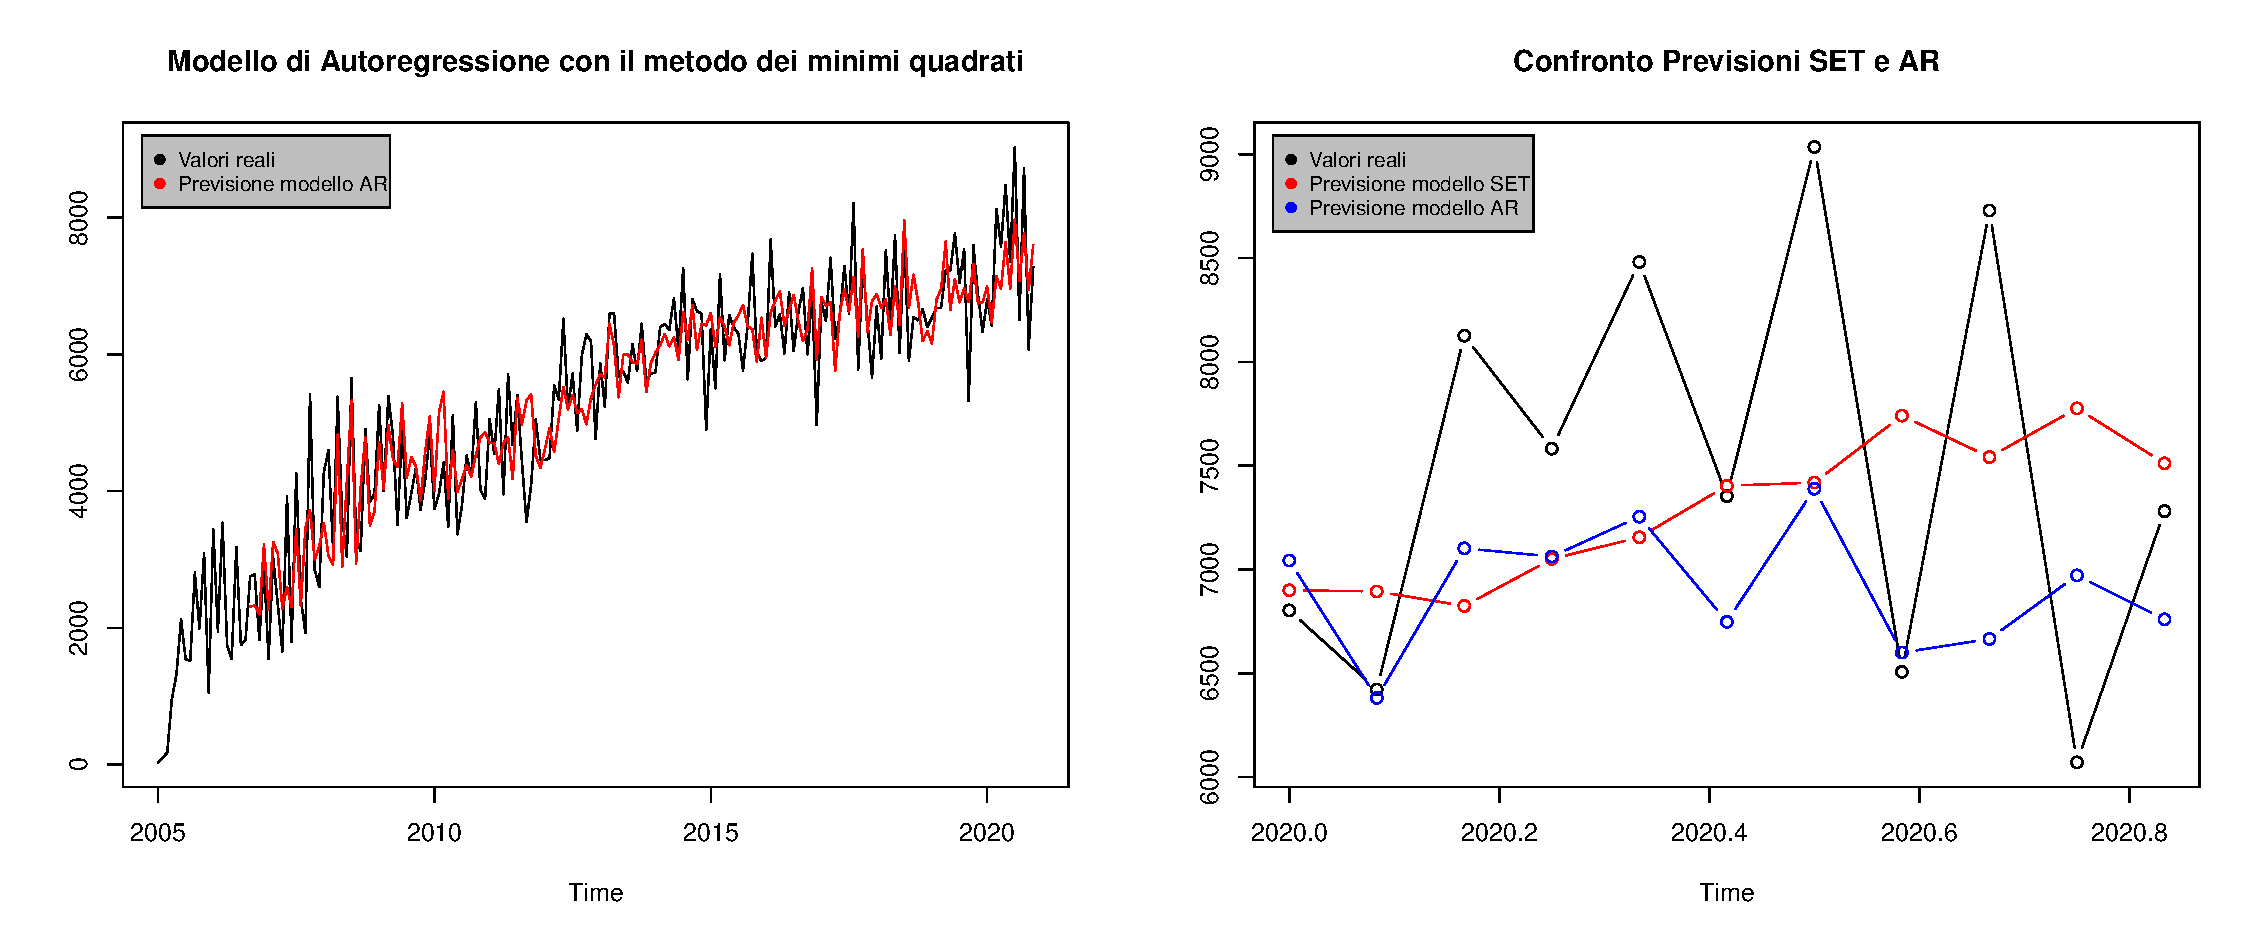
\includegraphics[scale=0.56]{imgs/AR_plot_test.pdf}
	\vspace{-0.9cm}
\end{figure}
\begin{figure}[H]
	\hspace{-2.5cm}
	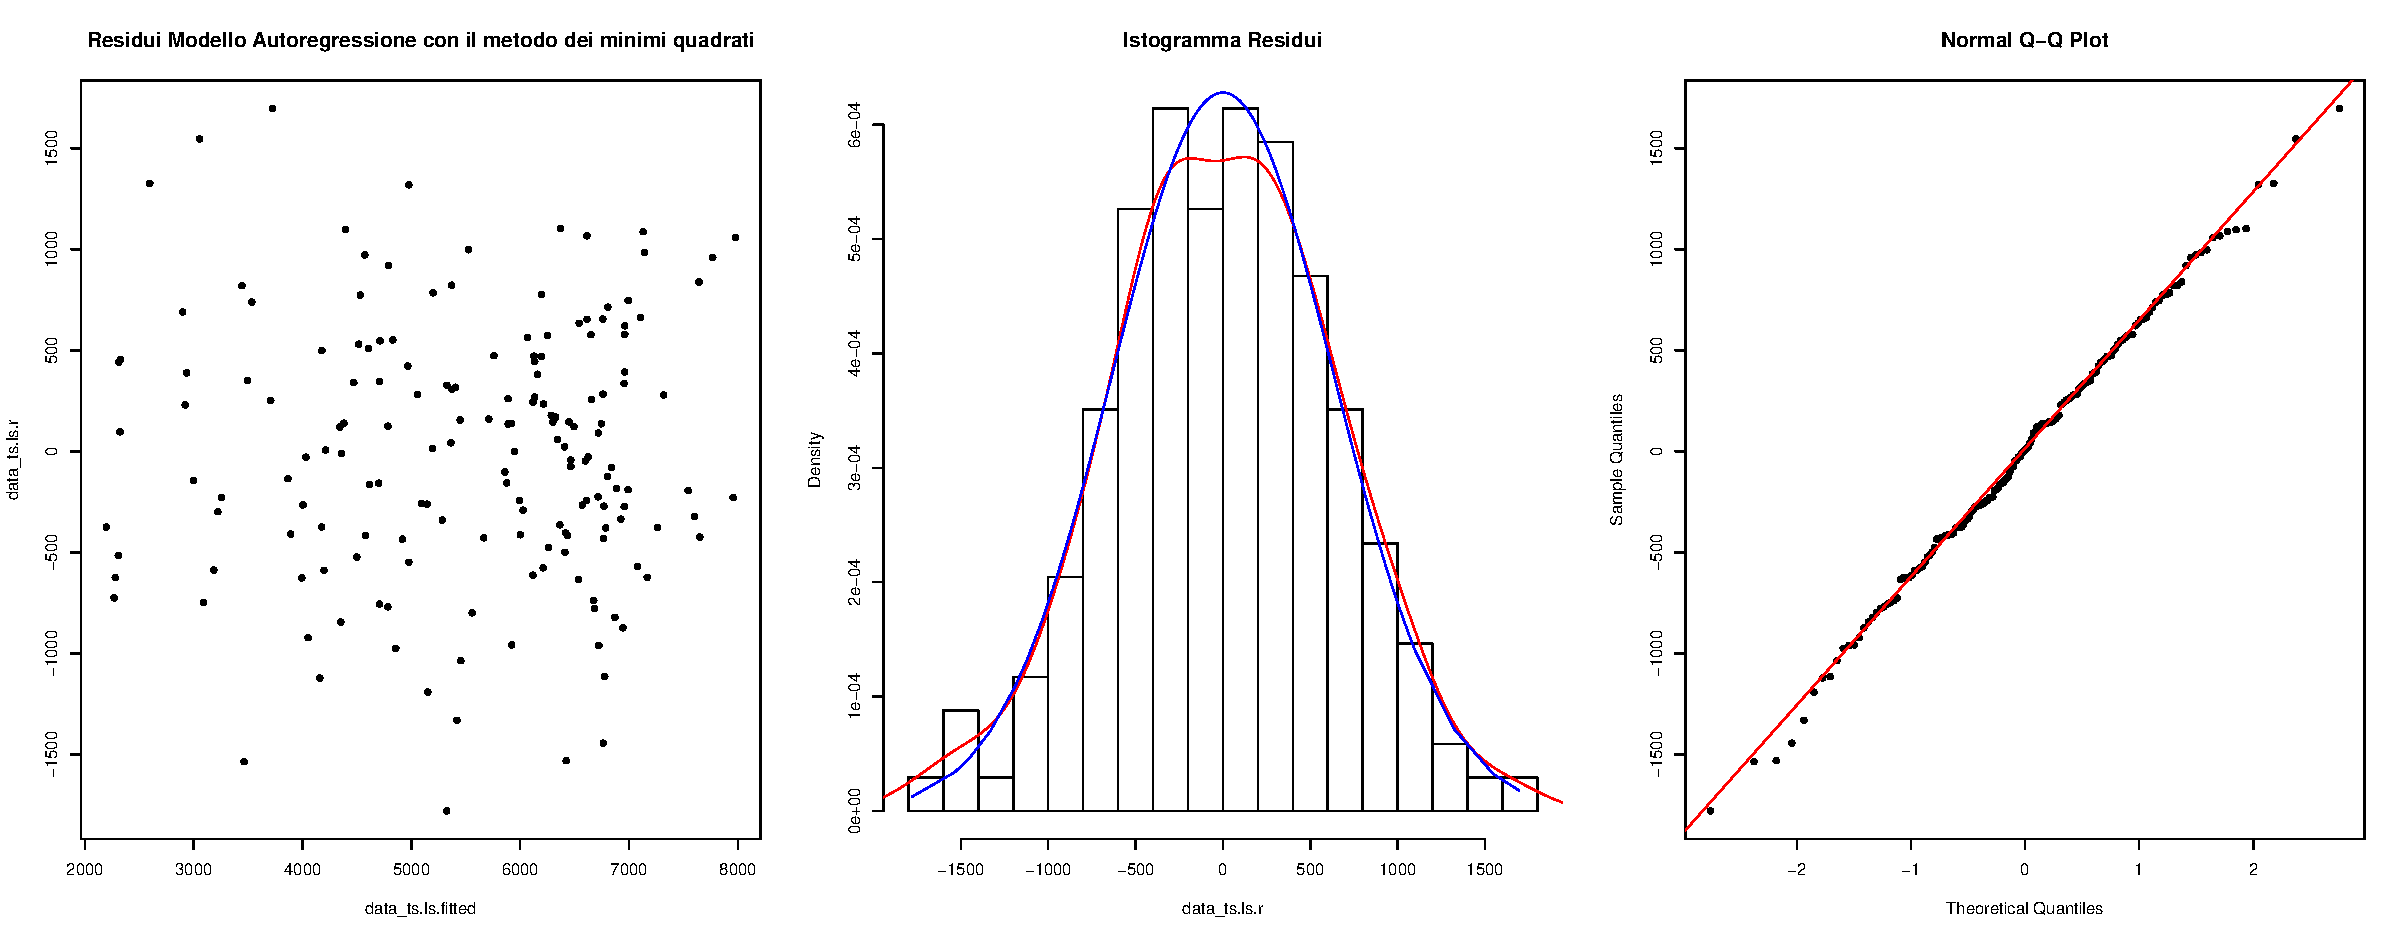
\includegraphics[scale=0.51]{imgs/AR_residuals.pdf}
	\vspace{-1.0cm}
\end{figure}

\section{Conclusione}
Certamente ci sarebbe da approfondire maggiormente i modelli di tipo
autoregressivo che, come ho sottolineato precedentemente, potrebbero darci una
mano a catturare quella parte del fenomeno che ha un comportamento aleatorio e
che porta ad avere una stagionalit\`a che evolve in maniera molto rapida.\\
\\
Ho tratto le conclusioni al termine di ogni fase di analisi. Evito pertanto di
allungare ulteriormente la relazione riassumendole nuovamente.
\end{document}
